\documentclass[fleqn,usenatbib,useAMS]{mnras}

\usepackage{graphicx}	% Including figure files
\usepackage{amsmath}	% Advanced maths commands
\usepackage{amssymb}	% Extra maths symbols
\usepackage{multicol}        % Multi-column entries in tables
\usepackage{bm}		% Bold maths symbols, including upright Greek
\usepackage{pdflscape}	% Landscape pages
\newcommand{\kms}{\,km\,s$^{-1}$} % kilometres per second
\newcommand{\bibtex}{\textsc{Bib}\!\TeX} % bibtex. Not quite the correct typesetting, but close enough

\usepackage[T1]{fontenc}
\usepackage{ae,aecompl}


%\usepackage{newtxtext,newtxmath}

%\documentclass[fleqn,usenatbib]{mnras}
%\usepackage{newtxtext,newtxmath}
%\usepackage[T1]{fontenc}

\usepackage{bigints}    %larger integrals
\usepackage{units}
\usepackage{tabularx}
\usepackage{cleveref}
\crefformat{section}{\S#2#1#3} % see manual of cleveref, section 8.2.1
\crefformat{subsection}{\S#2#1#3}
\crefformat{subsubsection}{\S#2#1#3}
%%%%%%%%%%%%%%%%%%%%%%%%%%%%%%%%%%%%%%%%%%%%%%%%%%

\usepackage{ulem}
\usepackage[dvipsnames]{xcolor}
\newcommand{\mjv}{\textcolor{cyan}}
\newcommand{\edit}{\textcolor{red}}
\newcommand{\Referee}{\textcolor{red}}
%%%%%%%%%%%%%%%%%%%%%%%%%%%%%%%%%%%%%%%%%%%%%%%%%%

\newcommand{\be}{\begin{equation}}
\newcommand{\ee}{\end{equation}}
\newcommand{\ba}{\begin{eqnarray}}
\newcommand{\ea}{\end{eqnarray}}
\newcommand{\mperh}{\,h^{-1}\,{\rm Mpc}}
\newcommand{\hperm}{\,h\,{\rm Mpc}^{-1}}
\newcommand{\todo}[1]{{\em \textcolour{red}{ #1}}}
\newcommand{\lang}{\langle}
\newcommand{\ra}{\rangle}
\newcommand{\vc}{\bm{c}}
\newcommand{\va}{\bm{a}(z)}
\newcommand{\vb}{\bm{b}(z)}
\newcommand{\vCo}{\bm{C}_{\rm obs}}
\newcommand{\vCoi}{\bm{C}_{\rm obs}^{-1}}
\newcommand{\vCi}{\bm{C}_{\rm int}(z)}
\newcommand{\vCii}{\bm{C}_{\rm int}^{-1}(z)}
\newcommand{\vCt}{\bm{C}_{\rm tot}(z)}
\newcommand{\vCti}{\bm{C}_{\rm tot}^{-1}(z)}
\newcommand{\ep}{\epsilon}
\newcommand{\pars}{\vec{\theta}}
\newcommand{\dev}{\mathrm{d}}
\newcommand{\mstar}{h^{-1}M_\odot}
\newcommand{\mrefz}{m_{i, \mathrm{ref}}}
\newcommand{\mi}{m_{i}}
\newcommand{\dense}{\mathtt{dense}}
\newcommand{\lum}{\mathtt{luminous}}
\newcommand{\dk}{\boldsymbol{w}_{g}^{(k)}}
\newcommand{\dg}{\boldsymbol{\gamma}_{t}}
\newcommand{\dbar}{\overline{\boldsymbol{w}_{g}}}
\newcommand{\njk}{N_{\rm JK}}
\newcommand{\healpix}{\mathtt{HEALPIX}}

%%%%%%%%%%%%%%%%%%% TITLE PAGE %%%%%%%%%%%%%%%%%%%

\title[KiDS DR4 LRG clustering]{Clustering of red-sequence galaxies in the fourth data release of the Kilo Degree Survey}


\author[M. Vakili et al.]{
Mohammadjavad Vakili$^{1}$\thanks{E-mail: vakili@mail.strw.leidenuniv.nl}, KiDS Collaboration\\
% List of institutions
$^{1}$Leiden Observatory, Leiden University, Leiden, Netherlands
}

% These dates will be filled out by the publisher
\date{Accepted XXX. Received YYY; in original form ZZZ}

% Enter the current year, for the copyright statements etc.
\pubyear{2018}

% Don't change these lines
%FIXME 
%\hypersetup{draft}

\begin{document}
\label{firstpage}
\pagerange{\pageref{firstpage}--\pageref{lastpage}}
\maketitle

% Abstract of the paper
\begin{abstract}

We present a sample of luminous red-sequence galaxies for studying the large-scale structure in the Kilo-Degree Survey fourth data release. The selected galaxies are well-described by a red-sequence template, a data-driven model of the color-magnitude relation as a function of redshift. In this work, the red-sequence template is calibrated using the broad-band optical+NIR photometry of KiDS-VIKIING and the overlapping spectroscopic datasets. The selection process involves estimating the red-sequence redshifts, their corresponding uncertainties, assessment of the purity of the sample, and computing the redshift distributions in tomographic bins. Then we inspect the correlation between the observed number density of these galaxies and the survey properties. In order to tackle these systematic dependencies, We provide a recipe based on reweighting the galaxies. Subsequently, we measure the angular two-point correlation function of these galaxies in tomographic bins. Finally, we estimate the linear bias of these galaxies in a blind fashion. 

\end{abstract}

% Select between one and six entries from the list of approved keywords.
% Don't make up new ones.
\begin{keywords}
galaxies: distances and redshifts, gravitational lensing: weak, methods: data analysis, methods: statistical
\end{keywords}
%\textbf{}\clearpage
%%%%%%%%%%%%%%%%%%%%%%%%%%%%%%%%%%%%%%%%%%%%%%%%%%

%%%%%%%%%%%%%%%%% BODY OF PAPER %%%%%%%%%%%%%%%%%%

\section{Introduction}

The Kilo Degree Survey (KiDS) is an optical galaxy survey primarily designed to map the large scale structure by studying the weak gravitational lensing of galaxies (\citealt{kuijken2015, kuijken2019}). This is done by measuring the correlation between the distortion of the shapes of distant galaxies (\citealt{hendrick2017,hendrik2018}). These correlations are then compared to the predictions of cosmological simulations to test cosmological models (\citealt{heymans2013,jee2016,hendrick2017,joudaki2017,troxel2017,joudaki2019, hikage2019}). 

However, the full constraining potential of weak lensing studies can only be realized through the joint analysis of the cosmic shear of back ground galaxies and the positions of foreground galaxies with robust distance estimates. This involves measuring the correlation between the cosmic shear estimates of the background galaxies, the correlation between the positions of foreground galaxies, and eventually the cross-correlation between the cosmic shear of background galaxies and the positions of foreground galaxies (\citealt{cacciato2013, cosmolike, des_y1_cosmology, elvin2017, edo2018, prat2017}). 

The advantages of such combined analyses are two-folded: obtaining tighter constraints on cosmological parameters and the possible extensions to the standard model of cosmology, and offering a venue for mitigation of a range of observational and theoretical uncertainties such as photometric redshift uncertainties and intrinsic alignments (\citealt{edo2016, joudaki2018, sam2019}). In this work, we focus on selection of a sample of galaxies with robust estimates of redshift as well as measuring their angular two-point correlation function in slices of redshift. 

Following the work of \citet{vakili2019} we construct a sample of red-sequence galaxies by taking advantage of the fact that at any given redshift, the distribution of these galaxies in the colour-magnitude space follows a straight line --- with some intrinsic scatter --- known as the red-sequence ridge-line \citep[e.g.][]{bower1992,ellis1997,gladders1998,stanford1998}. 

The redshift-dependent distribution of the red-sequence galaxies in the colour-magnitude space allows us to select these galaxies with the broad-band photometry of the imaging surveys (\citealt{gladders_yee2000,hao2009,redmap_sdss,rozo2016,elvin2017,oguri2018,vakili2019}). This can be achived with a data-driven model of the color-magnitude relation of the red-sequence galaxies as a function of redshift. In this work, we construct this data-driven model with the multi-band photometry of the KiDS DR4 (\citealt{kuijken2019}). In particular, we make use of the KiDS OmegaCAM $ugri$ optical bandpasses as well as the VIKING $Z$ bandpass.  

The model is calibrated with a set of spectroscopic redshifts obtained by four spectroscopic datasets, including SDSS DR13 (\citealt{sdss_dr13}), GAMA (\citealt{driver2011}), 2dFLenS (\citealt{blake2016}), and the GAMA reanalysis of the redshifts in G10-COSMOS region (hereafter G10-COSMOS \citealt{davis2015}). 

Following the $\textsc{redMagiC}$ prescription (\citealt{rozo2016}), we impose a set of luminosity cuts and constant comoving densities, and we construct two samples of luminous red galaxies suitable for galaxy clustering and galaxy-galaxy lensing measurements. The main differences between the method described in this work and the previous work of \citet{vakili2019} are: the inclusion of the VIKING $Z$-band magnitudes in the red-sequence template, and the inclusion of the G10-COSMOS in spectroscopic calibration of the model. We also use the VIKING $K_{\rm s}$ band to assess the purity of the sample selected based on the red-sequence template.  



Furthermore, we make use of the VIKING $K_{\rm s}$-band magnitudes to investigate the purity of the selected samples with different luminosity thresholds. Given the purity of the samples and the variable depth of the survey, we choose the redshift reaches of the dense and the luminous samples. The redshift reach of each sample is chosen such that the sample remains nearly pure and nearly volume-limited below that redshift. Afterwards, we divide the galaxy sample into four tomographic redshift bins between 0.15 and 0.8, with the first three redshift bins comprising the dense galaxy sample and the last bin consisting of the galaxies in the luminous sample. 

Given that the galaxy clustering measures the probability, in excess of randoms, of finding pair of galaxies at a given angular or physical separation, accounting for the impact of survey properties on the galaxy density variations across the survey requires a careful treatment. The properties as well as the observing strategies of the galaxy surveys can influence the detection of galaxies as well as the selection process of any galaxy sample in the survey \citep[e.g.][]{alam2017,kwan2017,ross2017,elvin2017,crocce2019,kalus2019}. These properties include the variable depth of the survey in the multiple bandpasses, the seeing, etc. Furthermore, the on-sky galaxy density variations are susceptible to star density variations across the survey as well as the galactic extinction (\citealt{ignacio2018,rezaie2019}). 

In this investigation, we follow the newly developed technique based on self-organizing-maps (\citealt{johntson2019}) to produce sets of random points that ingest the correlation of galaxy number densities with the survey systematic properties. We demonstrate the performance of the random points in terms of mitigating the galaxy-survey systematic correlations. Lastly, we compute the two-point correlation function and assuming a linear galaxy bias model and a nonlinear matter power spectrum at fixed cosmology, we provide theoretical fits to the compute angular clustering measurements in different tomographic bins. 

This paper is structured as follows. The data, both photometric and spectroscopic, are described in Section~\ref{sec:data}. In Section~\ref{sec:selection} we discuss the sample selection and the photometric redshifts. We then present the galaxy-density systematic correlations, production of randoms, and the performance of randoms in Section~\ref{sec:systematic}. In Section~\ref{sec:clustering} we present the computed two-point correlation functions as well as the theoretical fits.
Finally, we summarize and conclude in Section~\ref{sec:summary}. 

%Note that calculating the comoving densities and distances requires specifying a cosmology. In this work, we assume a flat $\Lambda$CDM cosmology with $\Omega_{m} = 0.3$ and $h=1.0$ \footnote{This is the convention used by \citet{redmap_sdss} in constructing the SDSS redMaPPer catalogue.}. All distances (comoving densities) are quoted in units of $h^{-1}\; \mathrm{Mpc}$ ($h^{3} \; \mathrm{Mpc}^{-3}$) respectively. Also note that the luminosity ratios used for selection of the red galaxies are not sensitive to the choice of $h$ and in this work and we always work with luminosity ratios. Whenever magnitudes are used, they will be provided in the AB system.

\section{Data}\label{sec:data}

\subsection{KiDS photometric data}\label{sec:kids}
The Kilo-degree Survey (KiDS, \citealt{kids}) is a wide 
imaging survey conducted with the OmegaCAM camera (\citealt{omegacam}) which is mounted on the VLT Survey Telescope (\citealt{vst}). This survey uses four broad-band filters ($ugri$) in the optical wavelengths. KiDS has targeted approximately 1350 deg$^2$ of the sky in two regions, one on the celestial equator and the other one in the South Galactic cap. 

KiDS broadband photometry in the optical is supplemented by the VISTA Kilo degree Infrared Galaxy (VIKING) survey (\citealt{irwin2004,lewis2010,Edge2013,Gonz2018}). The VIKING observations of nearly the same regions with the near infrared filters $ZYJHK_{s}$ significantly increase the wavelength coverage of KiDS, turning the KiDS dataset into a unique wide-field optical+NIR catalog suitable for cosmological analysis.

In this work we use the fourth KiDS data release (KiDS DR4 \citealt{kuijken2019}) which covers $1006$ deg$^{2}$ of the sky in 1006 tiles superseding the 440 tiles released in KiDS DR3 (\citealt{kids_dr3}). Reduction of the $ugri$ images was performed with the AstroWise pipeline (\citealt{omegacam}).  


The achieved 5$\sigma$ limiting AB magnitudes of the survey are 24.3, 25.1, 24.9, 23.8 in $2$ arcsec apertures in the $ugri$ bands respectively. For a thorough description of the KiDS data processing, we refer the readers to the data release paper (\citealt{kuijken2019}). 

The KiDS database includes magnitudes in the $r$-band derived by SExtractor (\citealt{sextractor}) such as \texttt{ISO} and \texttt{AUTO}. These magnitudes are determined directly from images with a variety of PSF values, they are therefore not optimal for our purposes where colours independent of such variations are needed. The KiDS data reduction involves however a post-processing procedure in which Gaussian Aperture and PSF (GAaP,~\citealt{gaap}) magnitudes are derived (\citealt{kuijken2015}). This procedure is performed in the following way. First, the PSF is homogenized across each individual coadd. Afterwards, a Gaussian-weighted aperture is used to measure the photometry. The size and shape of the aperture is determined by the object's length of the major axis, its length of the minor axis, and its orientation, all measured in the $r$-band. This procedure provides a set of magnitudes for all filters. 

The magnitudes used in this work are the zeropoint-calibrated and foreground dust extinction-corrected magnitudes\footnote{In the final catalogue and for each band, the zeropoint offsets ($\mathtt{ZPT}_{-}\mathtt{offset}_{-}\mathtt{band}$) and the Galactic extinction corrections ($\mathtt{EXT}_{-}\mathtt{SFD}_{-}\mathtt{band}$) based on \citet{schlegel98} are provided in separate columns.} 
denoted by $\; \mathtt{Mag}_{-}\mathtt{type}_{-}\mathtt{band}_{-}\mathtt{calib}$. 
In this notation, $\mathtt{calib}$ refers to the zeropoint-calibrated and extiction corrected magnitudes. $\mathtt{type}$ refers to the type of the magnitude, such as GAaP, $\mathtt{AUTO}$, or $\mathtt{ISO}$ magnitudes. Furthermore, $\mathtt{band}$ refers to the photometric band under consideration (i.e. $ugri$). The default magnitudes in KiDS are GAaP magnitudes, which were designed to provide accurate colours but underestimate total fluxes of large galaxies. Total fluxes are, however, needed in our LRG selection procedure to derive luminosities (see section~\ref{sec:overview}). Therefore, whenever galaxy fluxes are needed, we use $\mathtt{Mag}_{-}\mathtt{AUTO}_{-}\mathtt{band}_{-}\mathtt{calib}$ in our red-sequence modelling. 

For our choice of colour, GAaP colours are used as they have less scatter and bias than the colours derived from the $\mathtt{Mag}_{-}\mathtt{AUTO}_{-}\mathtt{band}_{-}\mathtt{calib}$ magnitudes. For the rest of this paper, we work with the calibrated $\mathtt{AUTO}$ $r$-band magnitude and GAaP colours. We emphasize that the GAaP procedure is intended to derive more accurate and less noisy estimates of colours for objects. In other words, the GAaP colours are less noisy than the colours estimated from the calibrated $\mathtt{AUTO}$ magnitudes ($\mathtt{Mag}_{-}\mathtt{AUTO}_{-}\mathtt{band}_{-}\mathtt{calib}$). We refer the readers to \citet{kuijken2015} and \citet{kids_dr3} for a more detailed discussion of the derivation of GAaP colours.

The nine-band photometric catalog is supplemented by a mask information
which removes the satellite tracks and other imaging artefacts such as stellar halos from the images. In KiDS DR4, the masking is carried out at the sub-exposure level, increasing the effective area of the coadd images.

\subsection{Spectroscopic data}\label{sec:spec}

In~\citet{vakili2019} we made use of the spectroscopic data of SDSS DR13, GAMA, and 2dFLenS. 
In addition to these data, we also take advantage of the KiDS deep field observation of the cosmos region, which overlaps with a number of spectroscopic campaigns such as zCOSMOS. 
In the COSMOS field we utilize the GAMA-G10 COSMOS spectrocopic data, which encompasses a wider magnitude range, albeit a much narrower area than the other spectroscopic data considered in this work. In what follows, we describe the spectroscopic datasets.

In this work, we exploit the overlap between the KiDS catalogue and a number of spectroscopic datasets. These datasets are used for the training and assessing the performance of the red-sequence template in selection and redshift estimation of LRGs.  
This procedure is explained in detail in our previous work (\citealt{vakili2019}). 

In addition to the datasets that we utilized in \citet{vakili2019}, we make use of the data
and it is applied to the overlap between the KiDS photometry and spectroscopic catalogues of galaxies in GAMA (\citealt{driver2011}) and SDSS DR13 (\citealt{sdss_dr13}). Later, for testing the performance of the redshifts estimated for the selected LRGs in section~\ref{sec:performance} we make use of the overlap between KiDS and the spectroscopic redshifts from SDSS, GAMA, as well as 2dFLenS (\citealt{blake2016}).
In what follows in the rest of this section, we provide a brief description of these spectroscopic catalogues.

We note that in general the spectroscopic samples such as those used here are systematically  brighter than the photometric data from which we will be selecting the LRGs. This means that bright galaxies are oversampled in the calibration data with respect to the faint end. However, this is not an issue for the LRG selection procedure of Sec.~\ref{sec:methodology}: what is needed is to have red spectroscopic galaxies to calibrate the red sequence template (colour-magnitude relation), which is approximately a straight line at each redshift. Consequently, one can use a relatively bright spectroscopic sample to estimate the colour-magnitude relation for fainter red galaxies.

The undersampling of the faint galaxies by overlapping spectroscopic data will be more of a problem for robust evaluation of photo-$z$ performance: at higher redshifts, the difference in average brightness between the full sample and the sample with spectroscopy is more significant than at the low-redshift, bright end, so the direct spec-$z$ -- photo-$z$ comparison may be indicating better performance than it actually is. We note however that the photo-$z$ error -- observational systematic trend presented in Sec.~\ref{sec:sys} will be still valid.

\subsubsection{GAMA}
Galaxy And Mass Assembly (GAMA,~\citealt{driver2011}) is a spectroscopic survey  which used the AAOmega spectrograph mounted on the Anglo-Australian Telescope. This survey spans five fields: G09, G12 and G15 on the celestial equators, and G02 and G23 on the Southern Galactic Cap. The only GAMA field outside the KiDS DR3 footprint is G02. The magnitude limited sample of GAMA is nearly complete down to $r=19.8$ mag for galaxies in the equatorial fields and down to $i=19.2$ mag for galaxies in the G23 region (\citealt{likse2015}). The GAMA spectra in the four fields that overlap with KiDS amount to a total of $\sim 230,000$ KiDS objects with high-quality spectroscopic redshifts with $\langle z \rangle = 0.23$. 

\subsubsection{SDSS}

The Sloan Digital Sky Survey (SDSS, \citealt{york2000}) is a photometric and spectroscopic survey of $14,555$ deg$^2$ of the sky encompassing more than one third of the celestial sphere using a dedicated 2.5-m telescope (\citealt{gunn2006}). In particular, we make use of the spectroscopic dataset from the Data Release 13 (DR13, \citealt{sdss_dr13}) of the SDSS-IV project. We only use objects with class `GALAXY'. 

The overlap between SDSS and KiDS in the equatorial fields above $\delta =-3$ ($\delta$ denotes the declination of objects on the sky) gives us $\sim 99252$ SDSS spectroscopic galaxies with KiDS photometry. However those with $r<19.8$ are mostly included in GAMA, and after removing the latter we are left with nearly $43,000$ unique SDSS spectroscopic galaxies with KiDS photometry. 

The SDSS-matched KiDS galaxies (after removing the overlap with GAMA) span higher redshifts than the GAMA-matched KiDS objects. This sample of galaxies mostly encompasses LRGs that are observed in the Baryonic Oscillation Spectroscopic Survey (BOSS, \citealt{dawson2013}) and the extended BOSS (eBOSS, \citealt{dawson2016}). This makes them ideal candidates for seed galaxies needed to estimate the red-sequence template as we seek to select galaxies that populate the same volume in the colour space as the SDSS LRGs do. 

\subsubsection{2dFLenS}
The 2-degree Field Lensing Survey (2dFLenS, \citealt{blake2016}) is a spectroscopic survey performed at the Australian Astronomical Observatory covering an area of 731 deg$^2$. By expanding the overlap with the KiDS field in the southern galactic cap, this survey aims to provide a dataset suitable for joint clustering and lensing analyses (\citealt{amon2018b,joudaki2018}), photometric redshift calibration (\citealt{johnson2017,wolf2017,kids_annz}), and lensing systematic tests (\citealt{amon2018a}).

In KiDS DR3 there are nearly $37461$ galaxies with 2dFLenS spectra. After excluding the galaxies in common with GAMA and SDSS, we have approximately $9,000$ unique 2dFLenS galaxies with KiDS photometry.

\subsubsection{GAMA-G10}

the Galaxy And Mass Assembly (GAMA) 10$^{\rm h}$ region (G10) (hereafter GAMA-G10) targets the data in the Cosmic Evolution Survey region (COSMOS). The GAMA-G10 consists of a curation and verification of approximately 16$k$ redshifts of bright galaxies in the COSMOS region (\citealt{davis2017}). Creation of this bright galaxy sample does not involve any target selection. All the 1d and the 2d spectra were process by the GAMA pipeline and were manually checked. Overall, the redshifts in this sample of bright galaxies are believed to be more robust than the redshifts obtained by the rest of the spectroscopic campaigns targeting the cosmos field \citep[e.g.][]{lily2009}.

\section{Sample selection}\label{sec:selection}

\subsection{Red-sequence model}

Several aspects of the selection procedure in this work are similar to what has been outlined  in~\citet{vakili2019}. In what follows we describe the main distinctions. Previously, we only took advantage of the KiDS optical photometry for our red-sequence model. In this work, we also include the VIKING $Z$ band in the red-sequence template. This allows the complexity of our model to be similar to that of~\citet{rozo2016} with the exception of the presence of the $u$ band.

In principle, one can also include the rest of the $YJHK_{\rm s}$ bandpasses of VIKING in the red-sequence model. However, we decided to exclude those bands in the modelling as they would increase the computational cost of the following steps: Selection of a set of seed galaxies (with spectroscopic redshifts) for estimating the parameters of the red-sequence template, and eventually computing the conditional probability of colors conditioned on the redshift and magnitudes for all the objects in the survey. 

As we discussed in Section~\ref{sec:data}, we make use the apparent AUTO magnitude in the $r$-band which is provided in KiDS DR4 as $\mathtt{MAG\_AUTO}$\footnote{The $\mathtt{AUTO}$ magnitudes are not provided in the rest of the KiDS-VIKING bands in KiDS DR4.} As discussed in Section~\ref{sec:data}, we make use of the GAaP $\{u-g,g-r,r-i,i-Z\}$ colors, which provide a more precise proxy for the colors of objects (\citealt{kuijken2019}). 

After evaluating $p(\boldsymbol{c}|m,z)$ and the red-sequence chi-squared $\chi^{2}_{\rm red}$, we proceed in a similar fashion as described in detail in \citet{rozo2016, vakili2019}. We construct two luminosity-threshold samples: the dense sample with $L>0.5 L_{\star}$ and a luminous sample with $L>L_{\star}$. 

For the luminous sample, we show the evolution of the GAaP colors with respect the estimated red-sequence redshifts in Figure~\ref{fig:cosmos_color}. We run our selection algorithm on the galaxies in the GAMA-G10 catalog. The selected red-sequence galaxies in GAMA-G10 are then used for the redshift calibration of the sample. In Figure~\ref{fig:cosmos_color}, the red points show the red-sequence galaxies with $L>L_{\star}$ in the GAMA-G10 COSMOS field. These galaxies are selected in a consistent manner and hence, they follow the redshift-dependent color distribution of the luminous red-sequence sample in KiDS DR4.

Moreover, we are interested in the morphological properties of the selected sample. We match the selected red-sequence galaxies in the GAMA-G10 field with the Zurich Structure and Morphology Catalog (\citealt{scarlata2007, sargent2007}). This catalog contains the best-fit parameters of the Single-Sersic GIM2D model applied to the COSMOS ACS catalog. We extract the $\mathtt{SERSIC\_N\_GIM2D}$ column of this catalog which represents the best-fit Sersic index. In Figure~\ref{fig:cosmos_sersic} the distribution of the Seric indices of red-sequence galaxies in GAMA G10 is shown in orange while that of all galaxies in the Zurich catalog is shown in blue. It is clear that Sersic indices of the selected red galaxies in GAMA-G10 tend to have higher values, consistent with the picture that these galaxies are well described by a bulge-dominated morphology.

\subsection{Purity and completeness}\label{sec:purity}

We furthermore assess the purity of the sample by inspecting the distribution of the selected objects in the $(r-Z, r-K_{\rm s})$ space. 
In particular we look at the distribution of the selected red-sequence galaxies and that of objects classified as high confidence star candidates in KiDS DR4. These star candidates are all the objects that meet this criterion: $\mathtt{SG\_FLAG}= 0$ \footnote{The $\mathtt{SG\_FLAG}$ parameter makes use of the size-peakiness relation of objects in order to determine whether they can be classified as star or not.}.
In Figure~\ref{fig:star_galaxy_I}, we show the distribution of red-sequence galaxies and high confidence stars in this two-dimensional color space. 
The left(right) panel of figure~\ref{fig:star_galaxy_I} shows this purity test for the selected objects in the dense(luminous) sample. On the other hand, the contours show the 68\% and 95\% of the distribution of high confidence stars in this two dimensional space. 

As apparent on the left panel of Figure~\ref{fig:star_galaxy_I}, there is significant overlap between the distribution of the colors of galaxies in the dense sample with $z_{\rm red}>0.6$ and the distribution of the colors of high confidence stars. On the contrary, there is a clear distinction between the color distribution of objects in the luminous sample and that of the high confidence stars. 

We use Support Vector Machines (hereafter SVM, see~\citealt{cristianini2000, scholkopf2000}) to estimate a boundary (a line) that maximizes the margin between the objects in the two classes in this two dimensional space. SVM's are a class of maximum margin  classifiers in which a decision boundary is chosen such that the margins between multiple classes are maximized (see \citealt{fadely2012, van2018} for some astrophysical applications of SVM).

In an $N$-dimensional Euclidean space, the decision boundary is an $(N-1)$-dimensional hyperplane which in our case is a line in the $(r-Z, r-K_{\rm s})$ space \footnote{In the case where a non-linear kernel for SVM is used, the $(N-1)$-dimensional hyperspace can be extended a $(N-1)$-dimensional manifold. Here we simply use a linear SVM since the two classes are linearly separable}. Figure~\ref{fig:star_galaxy_II} shows the decision boundary (red dashed line) as predicted by the SVM algorithm. The selected red-sequence galaxy candidates on the right hand side of the decision boundary---shown with red circles---are deemed miss-classified. Such objects are omitted from the red-sequence samples in order to maximize the purity of the sample shown in the right panel of Figure~\ref{fig:star_galaxy_II}. 

Evidently, the purity of the dense sample drops significantly for $z_{\rm red}>0.6$. On the other hand, the purity of the luminous sample remains nearly more than 90\% across the whole redshift range $<0.1<z_{\rm red}<0.8$. This significantly undermines the completeness of the dense sample for redshift above 0.6. 

\begin{table}
	\centering
	\caption{{\bf Photo-z tomography information:} 
    The tomographic bins, the mean redshifts and their corresponding 1-$\sigma$ uncertainties}
	
	\label{tab:pz}
	\begin{tabularx}{\columnwidth}{lccr} % four columns, alignment for each
		\hline
		Redshift bin &  Number of objects & $\langle z_{\rm red} \rangle$ & $\delta_{\langle z_{\rm red} \rangle}$ \\
		\hline
		$0.15 <z_{\rm red}<0.3$  & 32225  &  0.235 & $\pm$ 0.001  \\
		$0.3  <z_{\rm red}<0.45$ & 78086  &  0.388 & $\pm$ 0.003  \\
        $0.45 <z_{\rm red}<0.6$  & 124668  &  0.537 & $\pm$ 0.003  \\
        $0.6  <z_{\rm red}<0.8$  & 56880  &  0.712 & $\pm$ 0.008  \\
		\hline
	\end{tabularx}
\end{table}



Another important factor to take into consideration is the variable depth of survey in the bands used in the red-sequence model. Therefore, we inspect the distribution of the selected objects in a two dimensional space spanned by GAaP magnitude and the GAaP limiting magnitude.In particular, we aim to set the redshift reach of the samples such that the distribution of galaxies in this space is not bounded by the limiting magnitude of the survey. We carry out this investigation for the $ugriZ$ bands. For the $griZ$ bands the distribution of galaxies is not limited by the depth of the survey as long as a redshift cut of $z_{\rm red} < 0.6$ and $z_{\rm red} < 0.8$ are applied to the dense and the luminous samples respectively. 

This is demonstrated in Figure~\ref{fig:maglim_g} in which the distribution of galaxies is shown with the 2D purple histogram and the depth of the survey is indicated by the orange dashed line. For the $u$-band however, we note that even after applying the redshift cut of $z_{\rm red} < 0.6$ to the dense sample and $z_{\rm red} < 0.8$ to the luminous sample, both samples are bounded by the depth of the survey. The underlying reason of such limitation is that the red-sequence galaxies become faint in the $u$-band at high redshifts. This problem, amongst other things, is tackled in the next section~\ref{sec:systematic} where we discuss the various survey properties that can affect the observed number densities of galaxies.

\subsection{Photometric redshift distribution}

For our large scale structure study, we construct four redshift bins. 
In order to maximize the signal-to-noise ratio of the clustering as well as the tangential shear signals we make use of the dense sample as far as the purity and completeness considerations allow us (see section~\ref{sec:purity}). We construct three redshift bins with the dense ($L > 0.5 L_{\star}$) sample: $0.15<z_{\rm red}<0.3$, $0.3<z_{\rm red}<0.45$, $0.45<z_{\rm red}<0.6$; and finally one redshift bin with the luminous ($L > L_{\star}$) sample: $0.6<z_{\rm red}<0.8$.

For every galaxy in the catalog, we have computed a best estimate redshift $z_{\rm red}$ and a redshift uncertainty $\sigma_z$. This prompts us to compare the individual redshift probability distributions with the Normal distribution. We do so by comparing the distribution of the quantity $(z_{\rm red} - z_{\rm spec})/\sigma{z}$ and the Normal distribution in the four tomographic bins. We expect this assumption to hold if the individual redshift distributions with a Gaussian distribution centered on $\z_{\rm spec}$ (modulo some bias) and a scatter of $\sigma_{z}$. 

These distributions are shown in Figure~\ref{fig:pz} in four panels corresponding to the four redshift bins. In each panel, the blue histogram shows the distribution of the scaled redshift residuals while the orange curve shows a Normal distribution with a means set to the median of the scaled distribution and with a standard deviation set to the normalized median absolute deviation of the distribution. We note that the scatters are close to unity with the largest deviations from unity seen in the last two tomographic bins with a scatter of 0.944 and 1.021. Furthermore, the median of the distribution is largest in the last tomographic bin.

Overall, there seems to be an agreement between the distribution of the scaled redshift residuals and a Normal distribution with zero mean and a variance of unity. However, such approximation is not exact meaning that on average the redshift uncertainties are either over estimated (in the case of the first three redshift bins) or underestimated (in the case of the last tomographic bin) \footnote{We have furthermore done some experimentation with Gaussian mixture distributions. We have observed that the scaled residual redshift distributions are better described by multiple Gaussian distributions.}. 

In order to estimate the redshift distributions one can stack the individual redshift probability distribution functions assuming that each individual distribution is a Gaussian with the mean $z_{\rm red}$ and the standard deviation of $\sigma_{z}$. This is the approach undertaken by \citet{elvin2017}. We have decided not to follow this route for two reasons. Firstly, the Gaussian approximation for the individual redshift distributions is only an approximation, and more importantly, stacking the individual redshift distributions does not result in a mathematically correct distribution function for the population of galaxies. 

We use the Direct Redshift Calibration method (hereafter DIR) to estimate the redshift distributions (see~\citealt{lima2008, cunha2009}). In this, the redshift distribution of a photometric sample is estimated by reweighting the redshifts of galaxies in a spectroscopic sample. The reweighting is done such that the distribution of the magnitudes of galaxies in the spectroscopic sample is consistent with that of galaxies in the photometric sample. Similar to the prescription proposed by~\citealt{cunha2009} and \citealt{hendrik2018} in which reweighting is done with the $k$th nearest neighbors algorithm ($k$NN). 

In this approach for each spectroscopic galaxy in the 9 dimensional magnitude space, the distance to the fourth nearest neighbor in the same sample is measured. Afterwards, we count the number of galaxies in the photometric sample within the same radius in the nine-dimensional magnitude space. Finally, the weight of the spectroscopic galaxy is calculated by dividing the number of photometric galaxies within the 8-dimensional hypersphere by the total number of galaxies in the photometric sample. This density estimation technique has been previously followed by \citealt{nicola2019, zhou2020} in order to estimate the redshift distributions of galaxy clustering samples in the first data release of the Hyper Suprime-Cam Subaru Strategic Program (\citealt{hsc_dr1}) and the 8th data release of DESI Legacy Imaging Surveys (\citealt{desi_legacy}) respectively.   
It is important to note that this procedure is done for each redshift bin separately.

We estimate the sample variance of the redshift distribution from 1000 bootstrap samples of the spectroscopic galaxy catalog. The bootstrap samples provide us with an estimate of the uncertainty on the mean redshift of each tomographic bin. Figure~\ref{fig:pz2} shows the estimated DIR redshift distributions (shaded purple lines) as well as the stacked redshift pdfs (dashed red lines). The shaded orange area in each panel indicates the redshift boundaries of each bin, and the width of the purple line shows the bootstrap uncertainty on the estimated DIR distribution of the bin. The mean redshifts of the bins and their associated uncertainties are summarized in Table~\ref{tab:pz}



\section{Imaging systematics}\label{sec:systematic}

The observing conditions of large galaxy surveys such as KiDS are not homogeneous. 
The variable survey conditions can potentially affect the observed galaxy density and consequently can 
bias the cosmological inferences with these galaxy samples (\citealt{ross2012clustering, leistedt2014, leistedt2016mapping, zhai2017clustering, elvin2017, bautista2018sdss, crocce2019dark, DESI_systematic, rezaie2019, icaza2020clustering}). In what follows, first we describe the imaging systematics, and we will discuss their impact on the observed galaxy number densities and finally the mitigation strategies. 

\subsection{Systematic parameters}

We consider a range of photometric systematics with on-sky variations that can impact the variations of galaxy number densities. In total we consider 13 survey properties that we further pixellize using $\healpix$. We produce the $\healpix$ map of these properties with $n_{\rm side} = 256$. Moreover, we consider the galactic extinction in the $r$-band, and the star number density in the survey footprint. In what follows, we list the set of systematic properties considered in our investigation:

\begin{itemize}

  \item \textbf{Background count in the THELI images}: The background counts at the centroid positions of the objects in the THELI-processed $r$-band detection images. In KiDS DR4, the background count is provided as $\mathtt{BACKGROUND}$. Note that the THELI processed detection images are background subtracted. The $\mathtt{BACKGROUND}$ parameter simply returns the value of the residual sky background at the positions of objects. The healpix map of the background counts in shown in~ Figure\ref{fig:scatter_BackGr}.

  \item \textbf{Detection threshold above background}: This quantity is measured in units of counts and it is provided in the single-band source list as $\mathtt{THRESHOLD}$. 
  
  \item \textbf{Limiting magnitudes in 9 band}: The limiting GAaP magnitude attributes are provided in DR4 as $\mathtt{MAG}\textunderscore{}\mathtt{LIM}\textunderscore{} \mathtt{band}$, where $\mathtt{band} = \{u,g,r,i,Z,H,Y,J,K_{\rm s}\}$. 
  For each band the limitting magnitudes are evaluated on an object-by-object basis. At the position of a given object, the limitting GAaP magnitude corresponds to the 1-$\sigma$ GAaP flux error for the aperture of the source. The aperture size is set the optimal value of the minimum aperture $\mathtt{MIN}\textunderscore{}\mathtt{APER}$ in GAaP photometry. Thus, it depends on the pixel noise---in the Gaussianized image where the GAaP flux is measured---as well as the aperture size. This implies that the limitting magnitudes are indirectly dependent on the full-width-at half-maximum of the point spread function in the bandpass as well as the sky background counts.   
  
  \item \textbf{PSF FWHM in the $r$-band}: the PSF FWHM in the $r$-band measured in units of arcseconds. The PSF FWHM is calculated using the fallowing catalog entries: $\mathtt{PSFe1}$, $\mathtt{PSFe2}$, and $\mathtt{PSF \textunderscore{} Strehl \textunderscore{} ratio}$.
    
  \item \textbf{PSF ellipticity in the $r$-band}: the KiDS PSF ellipticity in the $r$-band. As discussed in \citet{kuijken2019}, both PSF ellipticity and the PSF FWHM in the $r$-band are small, allowing for benign imaging condition in the $r$-band which is used as the detection band in the KiDS photometry pipeline. 
  The PSF ellipticity quantity is computed from the $\mathtt{PSFe1}$, $\mathtt{PSFe2}$
  
  \item \textbf{Galactic dust extinction in the $r$-band}: This quantity is provided as $\mathtt{EXTINCTION\underscore{}r}$ in the nine-band catalog of KiDS DR4. The galactic extinction in the other bands are simply given by scaling of the extinction in the $r$-band.   
  
  \item \textbf{Star number density}: We determine the the stellar density from the pixellized number density map of bright stars in the second data release of GAIA (GAIA DR2). This is done by taking the GAIA stars with the $G$-band magnitude between 12 and 17. This is the magnitude range in which the GAIA DR2 G-band is complete (\citealt{gaia0,gaia1}). Note that only GAIA DR2 stars that lie in the KiDS $\mathtt{9bandnoAWr}$ mask are considered in the process of generating the map of stellar number densities. 
  
  It is worth noting that a number of parameters in the KiDS DR4 catalog are dedicated to star-galaxy separation. These include the $\mathtt{CLASS\textunderscore{}STAR}$
  parameter which is an output of the source extractor software, the $\mathtt{SG2DPHOT}$ parameter which is an internal KiDS star-galaxy classifier \citep[e.g.][]{kids_dr3, radovich2017}, and lastly the $\mathtt{SG\textunderscore{}FLAG}$ parameter which is derived based on an estimate of the size-peakiness relation of objects. Note that we have already excluded objects in our sample that are classified as high confidence stars according to the parameters $\mathtt{SG2DPHOT}$ and $\mathtt{SG\textunderscore{} FLAG}$. However, in order to reduce any impact of possible imperfections in the star-galaxy classification on our systematic tests, we decide to use a systematic map constructed from an external GAIA DR2 catalog with a pure and compete sample of stars. The healpix map of star nump densities is shown in Figure~\ref{fig:scatter_stardens}.
 
\end{itemize}

\subsection{The impact of photometric systematics}

In order to quantify such systematic-induced variations, we make pixellized on-sky maps of survey properties using the healpix framework (\citealt{healpix}) \footnote{In particular, we use healpy (\citealt{healpy2019}), a python library for handling and analyzing healpix maps.}. Similar to the works of \citet{ross2017, rezaie2019}, we construct the pixellized maps with the resolution of $N_{\rm side} = 256$. 

The systematic parameters considered in our investigation are not uncorrelated. Figure~\ref{fig:sys_sys_correlation} demonstrates the correlation between various systematic parameters in the survey namely: the limiting magnitude in the $u$-band, star number density, threshold, and the Background counts. For instance, there is a strong correlation between the limiting magnitude in the u band and the the star number density. Conversely, there is an anti-correlation between the background counts in the coadded $r$-band images and the star number density.

Due to the covariance between various imaging systematics, we inspect the variation of the observed galaxy number densities and the imaging systematics in the linear basis in which the covariance matrix between the systematic parameters is diagonal. The basis vectors of this space are the principal components of the imaging systematics. In such a basis, one can assess the variations between the observed galaxy number density and the different basis vectors independently. In particular, we inspect the variation of galaxy over-densities $\delta_{\rm gal} = N_{\rm gal}/\langle N_{\rm gal} \rangle$. Any deviation of this quantity with respect to unity will signal the impact of imaging systematics.\footnote{Note that alternatively, one can reformulate this by looking at the deviations of $N_{\rm gal}/N_{\rm random}$ (module some normalization) from one, where $N_{\rm random}$ is the number density of a set of uniformly distributed random points across the survey footprint (see \citep[e.g. ][]{bautista2018sdss, icaza2020clustering}).}   

The variation of the number density versus the systematic parameters is demonstrated in Figure~\ref{fig:sys_ng_correlation} where four rows correspond to the four tomographic bins in Table~\ref{tab:pz}. Note that the observed galaxy number density-systematic trends are shown with the orange errorbars. In each row, only the trends with considerable deviation from unity are shown. We note that the variations in the observed number density as a result of survey inhomogeneity changes depends on the galaxy sample under study,  with galaxies in different tomographic bins showing different sensitivities.

In this work we mitigate the impact of systematics by introducing a set of photometric weights to remove the variation of galaxy densities due to imaging systematics. This approach has been widely used in the literature in order to account for the impact os systematics: clustering of LRGs in SDSS BOSS (\citealt{ross2012clustering, ross2017clustering}), galaxy clustering in the Dark Energy Survey (\citealt{elvin2017,crocce2019dark}), DESI legacy survey (\citealt{DESI_systematic}), and clustering of LRGs in SDSS-eBOSS (\citealt{bautista2018sdss, icaza2020clustering}). 

Following the work of \citet{bautista2018sdss}, we introduce a set of photometric weights by assuming a linear relation between the pixellized observed galaxy overdensities and $\delta_{\rm gal} = N_{\rm gal}/\langle N_{\rm gal}\rangle$ and the set of pixellized systematic parameters. That is assuming $\boldsymbol{\delta}_{\rm gal} = \mathbf{Ws+b} + \mathbf{\mathrm{noise}}$. 

Additionally, we introduce an $L_{2}$ regularization to this linear regression problem in order to avoid overfitting. The advantage of such approach to that of \citet{ross2017clustering} is that it does not assume that there is no correlation between the systematic parameters. 

Alternatively, one can use self organizing maps (SOM, \citealt{kohonen1997}) to learn the systematic galaxy density modes due the variable survey properties and then generating a set of organized randoms mimicking the galaxy depletion pattern across the survey footprint (\citealt{som2020}). We have also tested this method and we have found that this method works best in correcting the systematic depletion in a galaxy sample with a higher number density than the galaxy sample in our study. 

Figure~\ref{fig:sys_ng_correlation} shows the variation of the number density with respect to the principal components of the systematic parameters before (shown in orange) and after (shown in blue) introducing the photometric weights. We note that after introducing the weights, the variations with respect to the systematics reduce significantly.

Furthermore, we compute the cross-correlation between the positions galaxies in the four redshift bins and a set of imaging systematics. Such cross-correlations have been used in~\citet{ho2012} and \citet{crocce2016galaxy} to find an unbiased estimate of the angular clustering in the presence of the systematics \footnote{This prescription relies on the assumption of the Gaussianity of the galaxy density field.}. Nonetheless, these cross-correlations can provide a useful diagnosis of the performance of the photometric weights in removing the systematic depletion of the galaxy densities. 

Cross-correlations between the galaxies and the $u$-band limiting magnitude (upper panel) and the background counts (lower panel) are shown in Figures~\ref{fig:xcorr_ulim_bkg}. It is evident that the cross-correlations after incorporating the photometric weights (blue points) are considerably reduced in comparison with the cross-correlations without the weights (orange points). Figure~\ref{fig:xcorr_threshold_ext} shows the cross-correlations with a different set of systematics: the detection threshold (upper panel) and the galactic extinction $E(B-V)$ (lower panel).

%We have not explored the effect of various observing conditions on the distribution of the physical properties of galaxies. Such effects can in principle generate systematic on-sky variations of the estimate host halo mass of galaxies in our sample. Such an effect can subsequently further complicate the cosmological analysis. This problem is exacerbated in a galaxy survey covering a larger area and can only be taken into account through a careful forward model approach which is outside the scope of this paper.  

\section{Galaxy Clustering}\label{sec:clustering}

\subsection{Theory}

Assuming a local linear galaxy bias, the galaxy overdensity $\delta_g$ can be related to the matter overdensity $\delta_m$ through a linear relation: $\delta_g = b_g \delta_m$, where the parameter $b_g$ is the linear bias parameter. Such assumption is expected to hold on sufficiently large scales \citep[e.g.][]{dvornik2018}, whereas on small scales, the nonlinear structure formation is best described by the more sophisticated halo model \citep[e.g. ][]{hand2017,vakili_hahn}.

For a population of galaxies described by a linear bias parameter $b_g$, and a redshift distribution of $n_g(z)$, and a nonlinear matter power-spectrum $P_{\delta}(k,z)$, one can predict the angular clustering of the galaxy sample.

\begin{eqnarray}
w_{g}(\theta) &=& b_g^2 \int \frac{l dl}{2\pi}J_{0}(l\theta)  \nonumber \\ 
            &\times& \int d\chi_{\rm cov} \Big[\frac{n_{g}(z)\frac{dz}{d\chi_{\rm cov}}}{\chi_{\rm cov}}\Big]^{2}P_{\rm NL}\Big(\frac{l+1/2}{\chi_{\rm cov}}; \; z\Big),                  
\label{eq:clustering_theory}
\end{eqnarray}
where $\chi_{\rm cov}$ is the comoving distance with a redshift dependence that itself depends on the choice of cosmology. The term $P_{NL}$ is the analytical nonlinear power spectrum which can be calculated using different recipes such as the halo model \citep[e.g. ][]{takahashi2012, mead2015, smith2019}, or emulation \citep[e.g.][]{emu2014}. We calculate the theoretical prediction (\ref{eq:clustering_theory}) for all four tomographic bins in our galaxy sample, each with their corresponding linear bias parameter $b^{(i)}_{g}$ and redshift distribution $n^{(i)}_{g}(z)$, where $i\in {1,2,3,4}$ corresponds to the tomographic bins defined in Table~\ref{tab:pz}.

Assuming a fixed cosmology, we estimate the linear bias parameters $\{b^{(i)}_{g}\}_{i=1}^{4}$ by fitting the theoretical prediction (\ref{eq:clustering_theory}) to the angular clustering measurements provided in Section~\ref{sec:measurement}. It is important to note that one major source of systematic in this theoretical prediction is the uncertainty on the mean of the redshift distributions $\{n_{g}^{(i)}(z)\}_{i=1}^{4}$. In order to mitigate the impact of such systematic, we assume that the estimated redshift distribution at each tomographic bin $n_{g}^{(i)}(z)$ is effectively given by shifting the unbiased redshift distribution $n_{g, \rm true}^{(i)}(z - \delta z^{(i)})$, where the parameter $\delta z^{(i)}$ is uncertainty on the mean of the redshift distribution of $i$-th redshift bin. In Section~\ref{sec:selection} we have estimated these redshift uncertainties. When constraining the galaxy bias parameters, we marginalize over the individual redshift uncertainties. 

\subsection{Clustering measurements}\label{sec:measurement}

Galaxy 2PCF is the probability in excess of random of finding a pair of galaxies within a given angular or physical separation. Given that we do not know the exact redshifts of the galaxies, we focus on computing the angular 2PCF which can be obtained by performing pair-counts in angular bins. The angular clustering can be measured using the Landy-Szalay estimator (\citealt{landy}):
\begin{equation}
    \hat{w}(\theta) = \frac{DD-2DR+RR}{RR},
\label{eq:landy}
\end{equation}
where $DD$ denotes the number of galaxy pairs within an angular separation bin centered at $\theta$, $DR$ denotes the number of galaxy-random pairs, and $RR$ denotes the number of random pairs. 

As discussed in Section~\ref{sec:systematic}, In each redshift bin, depending on the position of a given galaxy on the sky, a photometric weight is assigned to it. These weights are derived such that the on-sky variations of galaxy overdensity due to survey systematic properties are removed. In what follows in this section we compute two sets of angular 2PCF, one taking the photometric weights into account, and another without the photometric weights. 

Figure~\ref{fig:xi} shows the angular clustering measurements of LRGs at 4 tomographic bins, with the first three bins encompassing the galaxies in the dense (L> 0.5 * L_{\star}) sample and the last bin ($0.6<z<0.8$) encompassing the galaxies in the luminous (L> L_{\star}) sample. The clustering signal estimated using the photometric weights is shown by the blue data points and the signal estimated without the weights is shown by the blue data points. 

We estimate the measurement uncertainties using the jackknife resampling method (\citealt{norberg2009,oliver2016,singh2017,shirasaki2017}). 
In the jackknife method, the survey footprint is first divided into $N_{\mathrm{JK}}$ jackknife subregions of approximately equal area. 
Then for each subregion $k\in\{1,...,N_{\mathrm{JK}}\}$, the clustering data vector $\boldsymbol{w}_{g}^{(k)} = \langle w^{(k)}_{g}\rangle$ is measured by cutting out the $k$-th subregion and estimating the clustering signal of the rest of the survey footprint. Note that $\boldsymbol{w}_{g}^{(k)}$ is a vector which contains the 2PCF in all angular bins considered in this study. The jackknife estimator of the covariance matrix is then given by:
\be 
C_{\rm JK} = \frac{\njk - 1}{\njk}\sum_{k=1}^{\njk}\big(\dk-\dbar\big)^{T}\big(\dk-\dbar\big), 
\label{eq:jk}
\ee
where $\dbar$ is the mean of all $\boldsymbol{w}_{g}^{(k)}$ vectors. 


\subsection{Inference setup}

In order to fit the theoretical predictions of angular clustering to the measurements, we need to specify some choices. Assuming a fixed cosmology, we estimate the linear galaxy bias~(\ref{eq:clustering_theory}) of the red galaxies in the four different tomographic bins. These parameters are denoted by $\{b^{(1)}_g, \; b^{(2)}_g, \; b^{(3)}_g, \; b^{(4)}_g\}$. Furthermore, we keep our estimates of the photometric redshift distributions fixed. That is, we do not marginalize over photo-$z$ uncertainties. In our future 3x2pt analysis however, we will jointly constrain the cosmological parameters, linear galaxy bias, as well as photometric redshift uncertainties of our sample. 

Furthermore, we choose a flat LCDM model assuming $\Omega_m = 0.25, \;\Omega_{\Lambda} = 0.75, \; \Omega_b = 0.044, \; \sigma_{8} = 0.8, \; n_s = 0.95, \; h = 0.7$. Our choice is consistent with the MICE suite of cosmological simulations (\citealt{MICE1}) which itself is consistent with the best-fit flat LCDM cosmology given the WMAP5 data (\citealt{WMAP5}). 

In order to avoid confirmation bias we adopt the blinding scheme introduced in (\citealt{sellentin2019}). In this approach the blinded element of the inference pipeline is the inverse covariance matrix as oppsed to the data products (see for example \citealt{hendrick2017, hendrik2018}). The estimated inverse covariance matrix is changed by multiplication of a diagonal matrix to the Cholesky decomposition of the estimated inverse covariance matrix. The diagonal matrix is chosen such that the posterior distributions derived from the new inverse covariance matrix are shifted with the respect to those derived from the fiducial covariance matrix. 

\begin{eqnarray}
\hat{C^{-1}} &=& L^{T}L \\
             &\rightarrow& L^{T}B^{T}BL
\end{eqnarray}

The theoretical model summarized in equation~\ref{eq:clustering_theory} fails to capture the full complexity of galaxy-matter connection on small scales as it relies only on a simple linear deterministic treatment of galaxy bias. Therefore, we decide to apply a conservative cut on the comoving scales considered in our theoretical fittings. In particular, we adopt a cut at a comving scale of 8 $\mathrm{Mpc}h^{-1}$ which translates to the minimum angular scale (hereafter denoted by $\theta_{\rm min}$) of 30 arcmin for the first bin, 18.4 arcmin for the second bin, 14 arcmin for the third bin, and finally 11 arcmin for the last tomographic bin. The comoving distance is converted to angular scales assuming the flat LCDM cosmology discussed shortly above. Furthermore, the parameter $\theta_{\rm min}$ in each tomographic bin is calculated from the comoving distance at the mean redshift of the bin.


\section{Summary}\label{sec:summary} 


\section*{Acknowledgements}


\begin{figure*}
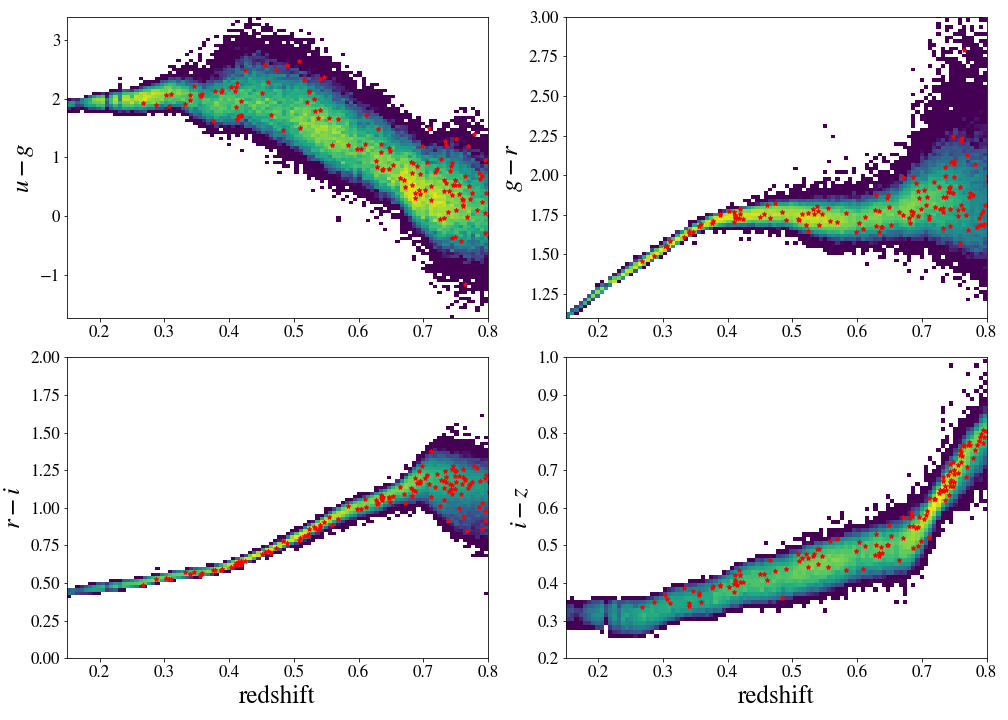
\includegraphics[width=\textwidth]{figures_tmp/cosmos_color.png}
\caption{\label{fig:cosmos_color}Distribution of the selected luminous red-sequence galaxies in 
the color space as a function of redshift. The COSMOS-G10 galaxies are shown in red dots.} 
\end{figure*}

\begin{figure}
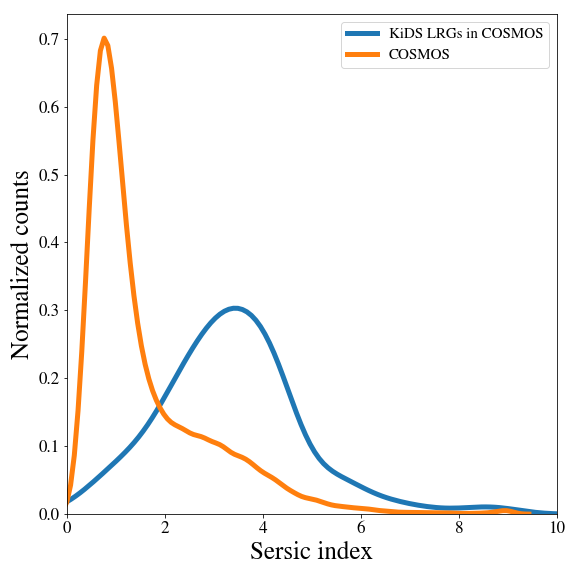
\includegraphics[width=\columnwidth]{figures_tmp/cosmos_sersic.png}
\caption{\label{fig:cosmos_sersic}Distribution of Sersic indices of LRG's in the COSMOS field.} 
\end{figure}


\begin{figure*}
\begin{tabular}{cc}
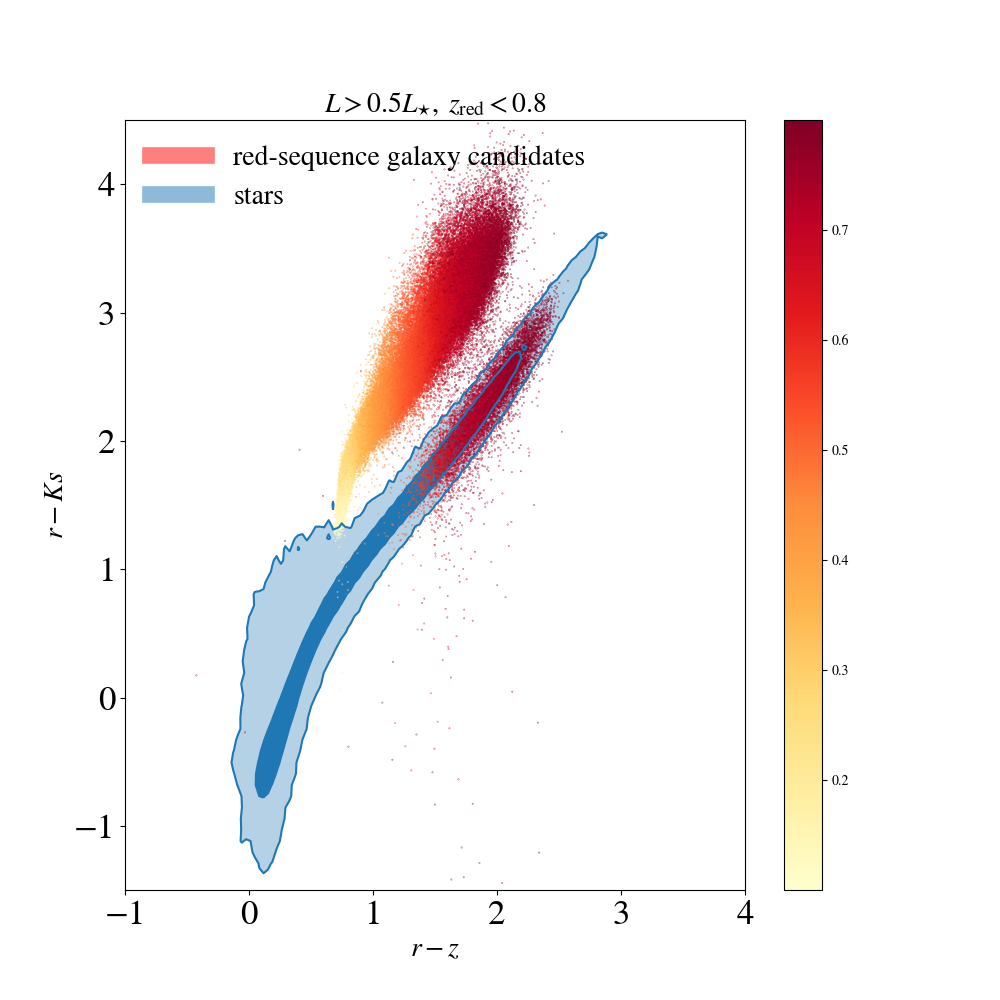
\includegraphics[width=0.5\textwidth]{figures_tmp/red_vs_star_dense.png}
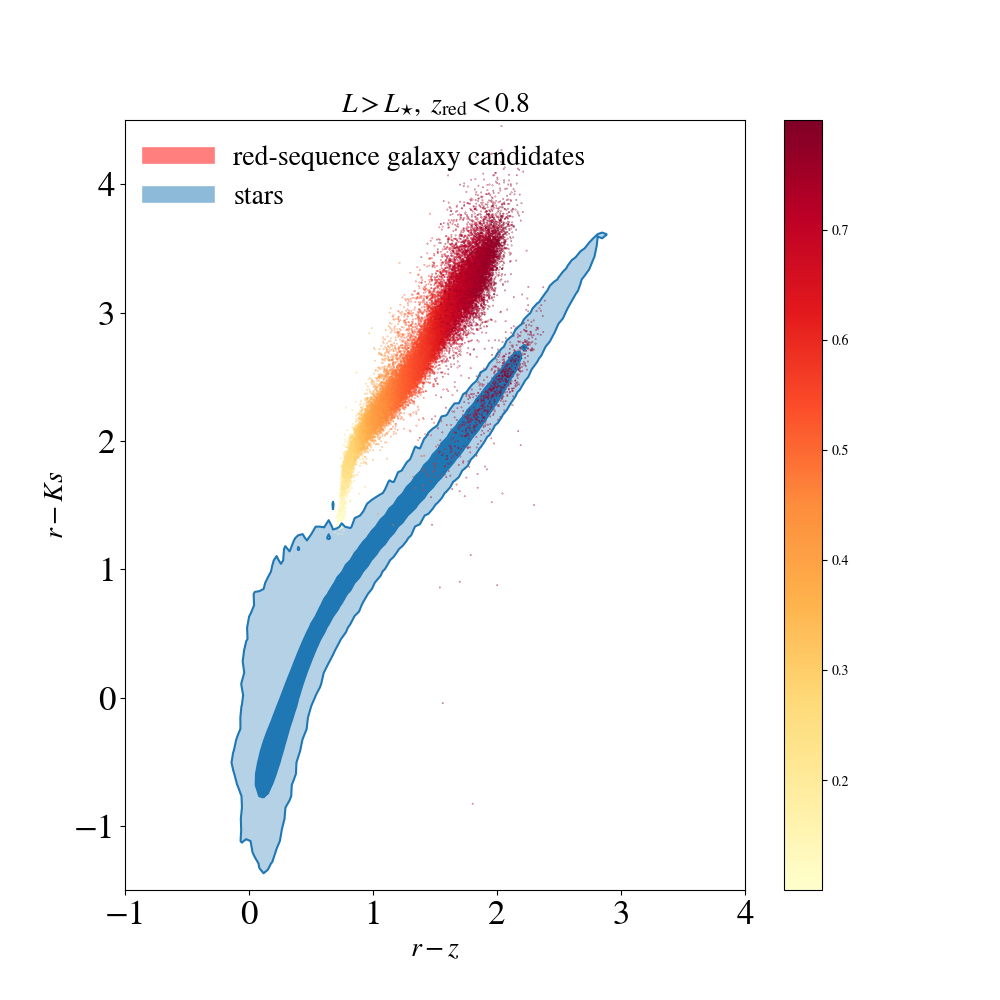
\includegraphics[width=0.5\textwidth]{figures_tmp/red_vs_star_lum.png}
\end{tabular}
\caption{\label{fig:star_galaxy_I} Demonstration of the use of optical+NIR colors for identification of likely stellar objects amongst the red-sequence galaxy candidate. Right Panel: At redshifts above $z_{\rm red}>0.4$ red-sequence galaxies (shown in red) and high confidence stars (shown in blue) reside in separated regions of the two-dimensional $(r-K_{\rm s}) \times (r-z)$ colors. Shown in pink dashed line is the support vector machine prediction of a boundary line between the two classes. The red-sequence candidates falling below the predicted boundary are marked by open circle and thus masked as likely stellar objects in the final catalog. Left Panel: Purity fraction of the dense  (green dashed line) and the luminous (orange dashed line) samples defined as the stellar contamination fraction subtracted from unity.} 
\end{figure*}


\begin{figure*}
\begin{tabular}{cc}
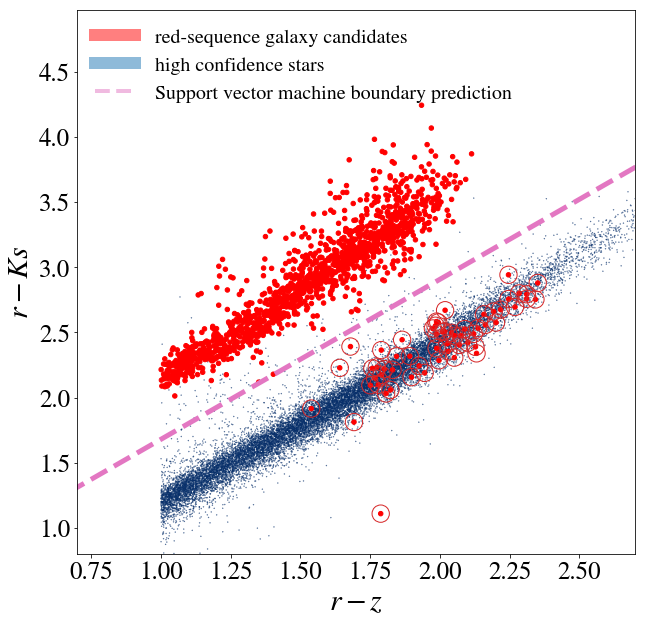
\includegraphics[width=0.5\textwidth]{figures_tmp/stars_SVM_lum.png}
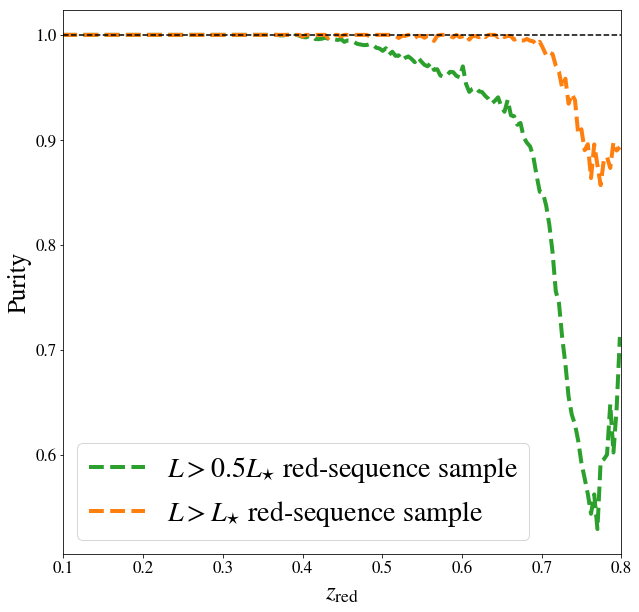
\includegraphics[width=0.5\textwidth]{figures_tmp/lrg_purity.png}
\end{tabular}
\caption{\label{fig:star_galaxy_II} Demonstration of the use of optical+NIR colors for identification of likely stellar objects amongst the red-sequence galaxy candidate. Right Panel: At redshifts above $z_{\rm red}>0.4$ red-sequence galaxies (shown in red) and high confidence stars (shown in blue) reside in separated regions of the two-dimensional $(r-K_{\rm s}) \times (r-z)$ colors. Shown in pink dashed line is the support vector machine prediction of a boundary line between the two classes. The red-sequence candidates falling below the predicted boundary are marked by open circle and thus masked as likely stellar objects in the final catalog. Left Panel: Purity fraction of the dense  (green dashed line) and the luminous (orange dashed line) samples defined as the stellar contamination fraction subtracted from unity.} 
\end{figure*}


\begin{figure*}
 
 \begin{tabular}{cc}
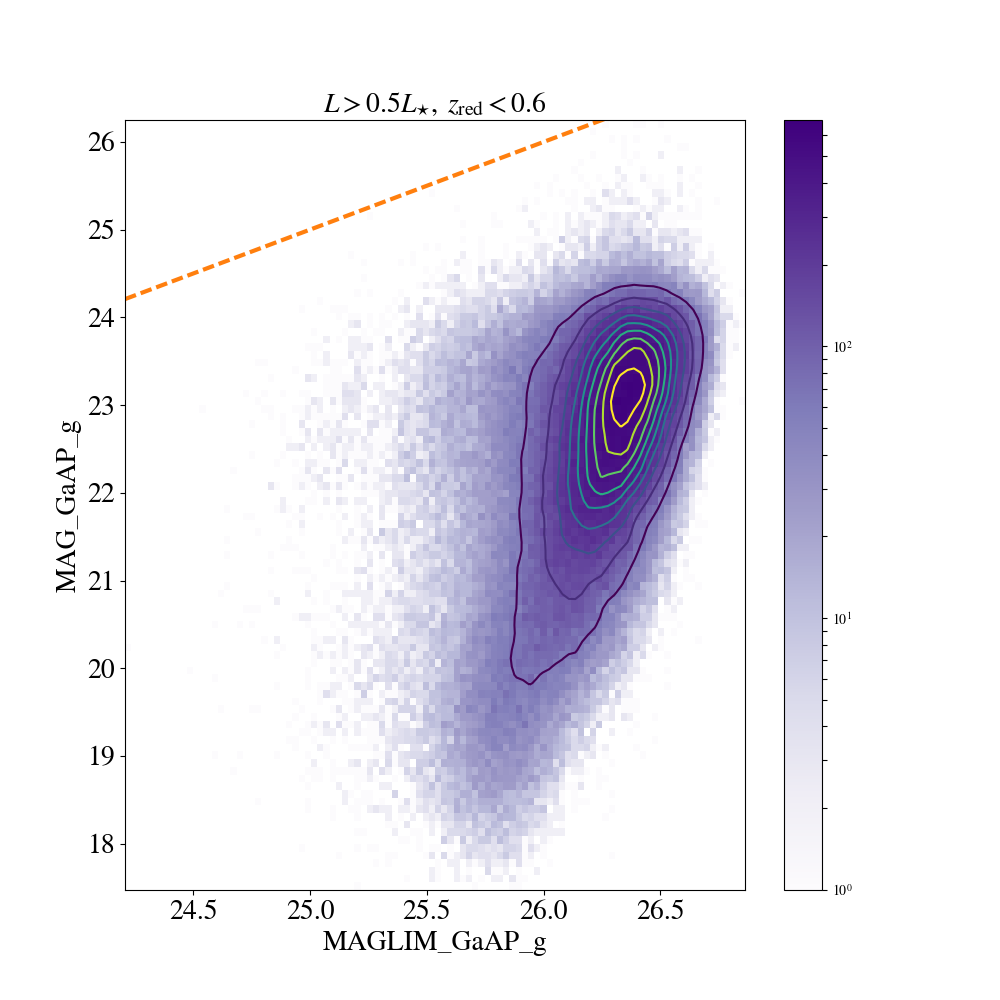
\includegraphics[width=0.5\textwidth]{figures_tmp/magg_lim_type_dense_zmax_0_6.png}
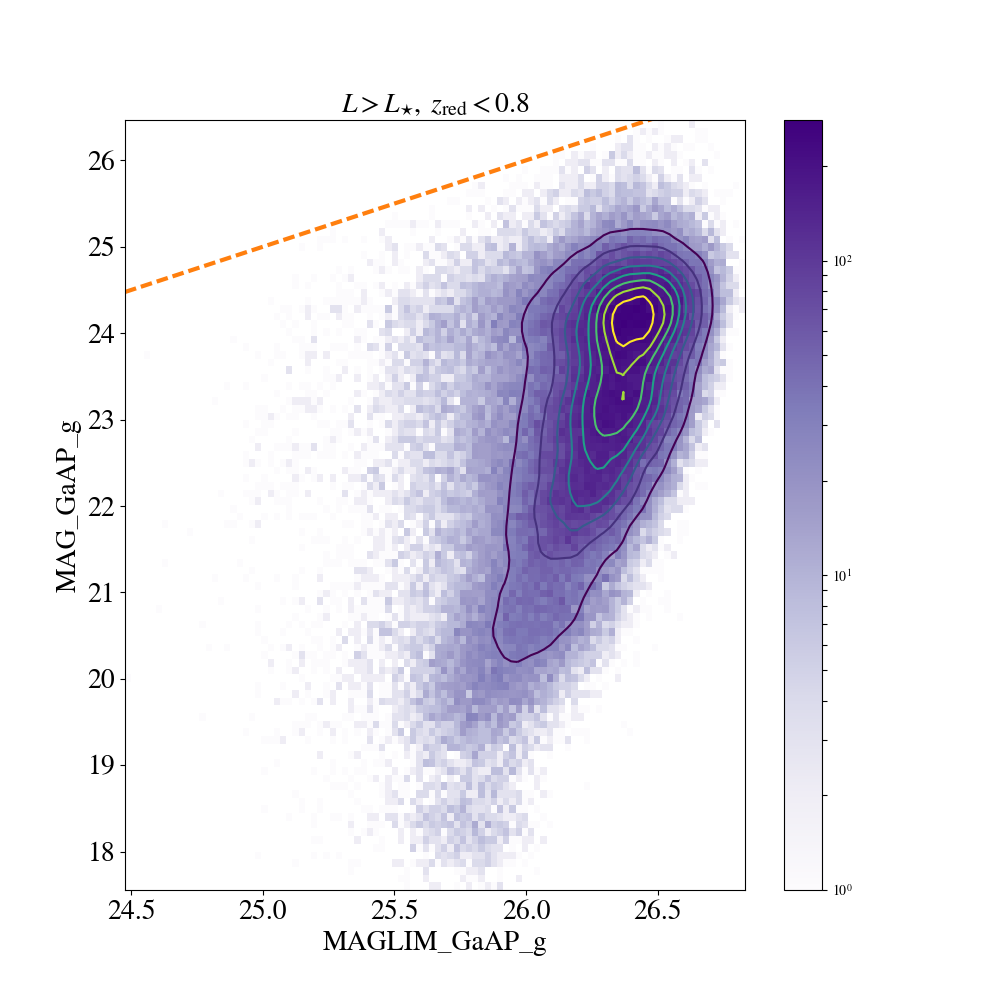
\includegraphics[width=0.5\textwidth]{figures_tmp/magg_lim_type_lum_zmax_0_8.png}
\end{tabular}
\caption{\label{fig:maglim_g} Demonstration of the distributions of the GaAP magnitudes and the limiting magnitudes in the $g$-band for the dense sample (left panel) and the luminous sample (right panel). In both figures the pixelised distributions and contours are color-coded by the number counts. Note that the maximum redshifts of the two samples, $z_{\rm red}=0.6$ (dense) sample and $z_{\rm red}=0.8$ (luminous) sample are chosen such that the samples remain volume-limited and not limited by the varying depth of the survey (shown with the dashed orange line in both panels).} 
\end{figure*}

\begin{figure*}
 
 \begin{tabular}{cc}
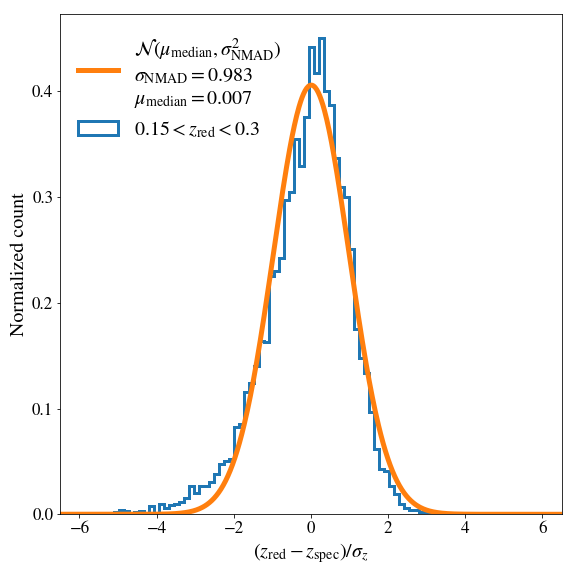
\includegraphics[width=0.5\textwidth]{figures_tmp/nz_normal_1.png}
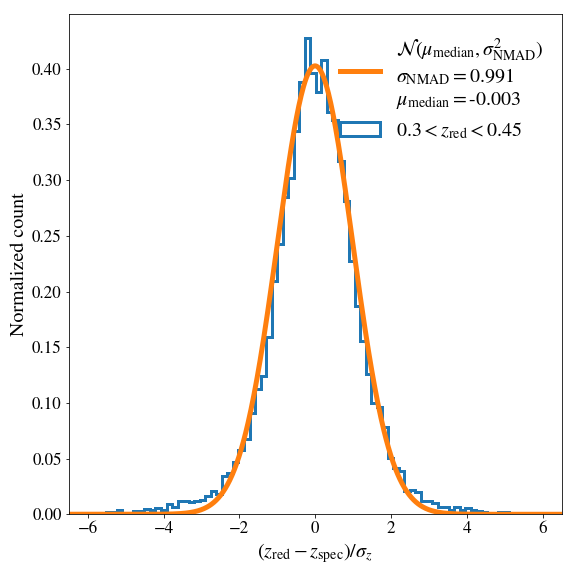
\includegraphics[width=0.5\textwidth]{figures_tmp/nz_normal_2.png}
\end{tabular}

 \begin{tabular}{cc}
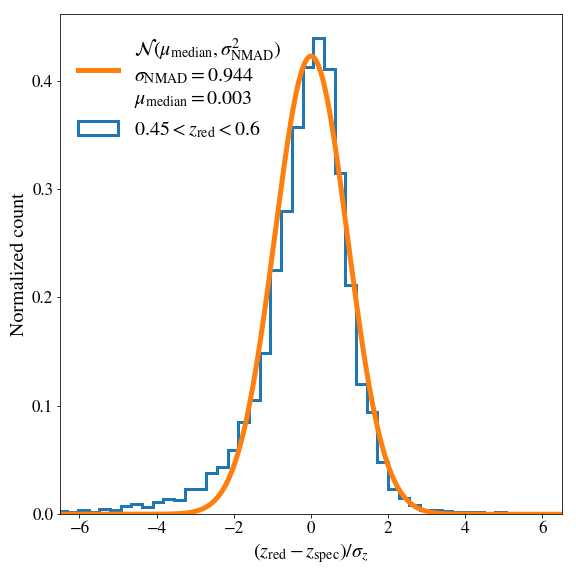
\includegraphics[width=0.5\textwidth]{figures_tmp/nz_normal_3.png}
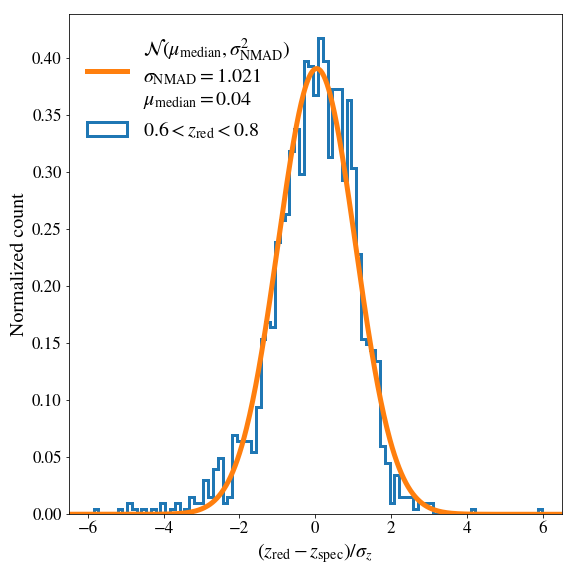
\includegraphics[width=0.5\textwidth]{figures_tmp/nz_normal_4.png}
\end{tabular}
\caption{\label{fig:pz} The Blue histogram shows the distribution of the offset between the red-sequence redshifts $z_{\rm red}$ and the spectroscopic redshifts $z_{\rm spec}$, weighted by their corresponding redshift uncertainties $\sigma_{z_{\rm red}}$. The orange solid line is a Gaussian distribution with zero mean and standard deviation of unity. This demonstrates that the a Gaussian distribution is a good description of the red-sequence redshift probability distribution functions of galaxies in the our sample of luminous red galaxies.} 
\end{figure*}


%\begin{figure}
%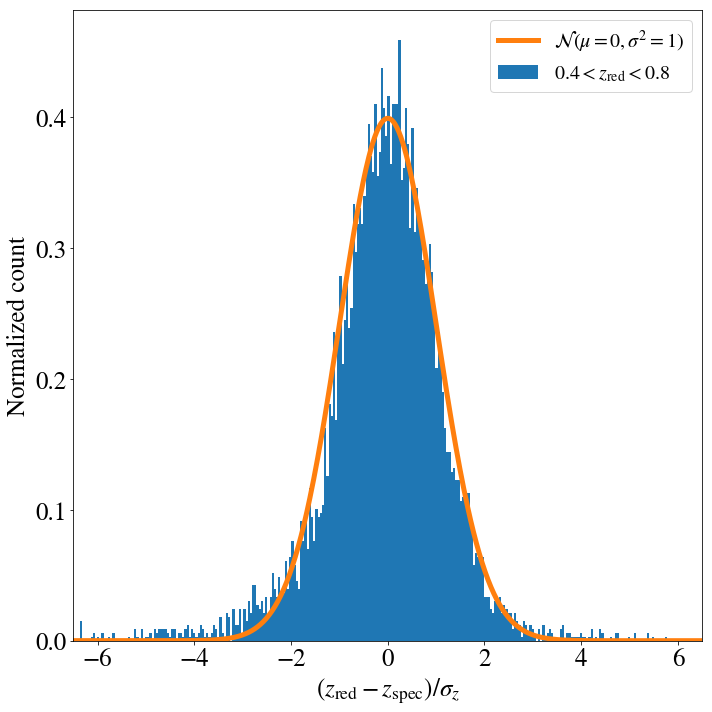
\includegraphics[width=\columnwidth]{figures_tmp/zerr_dist_2.png}
%\caption{\label{fig:pz} The Blue hisogram shows the distribution of the offset between the red-sequence redshifts $z_{\rm red}$ and the spectroscopic redshifts $z_{\rm spec}$, weighted by their corresponding redshift uncertainties $\sigma_{z_{\rm red}}$. The orange solid line is a Gaussian distribution with zero mean and standard deviation of unity. This demonstrates that the a Gaussian distribution is a good description of the red-sequence redshift probability distribution functions of galaxies in the our sample of luminous red galaxies.} 
%\end{figure}


%\begin{figure}
%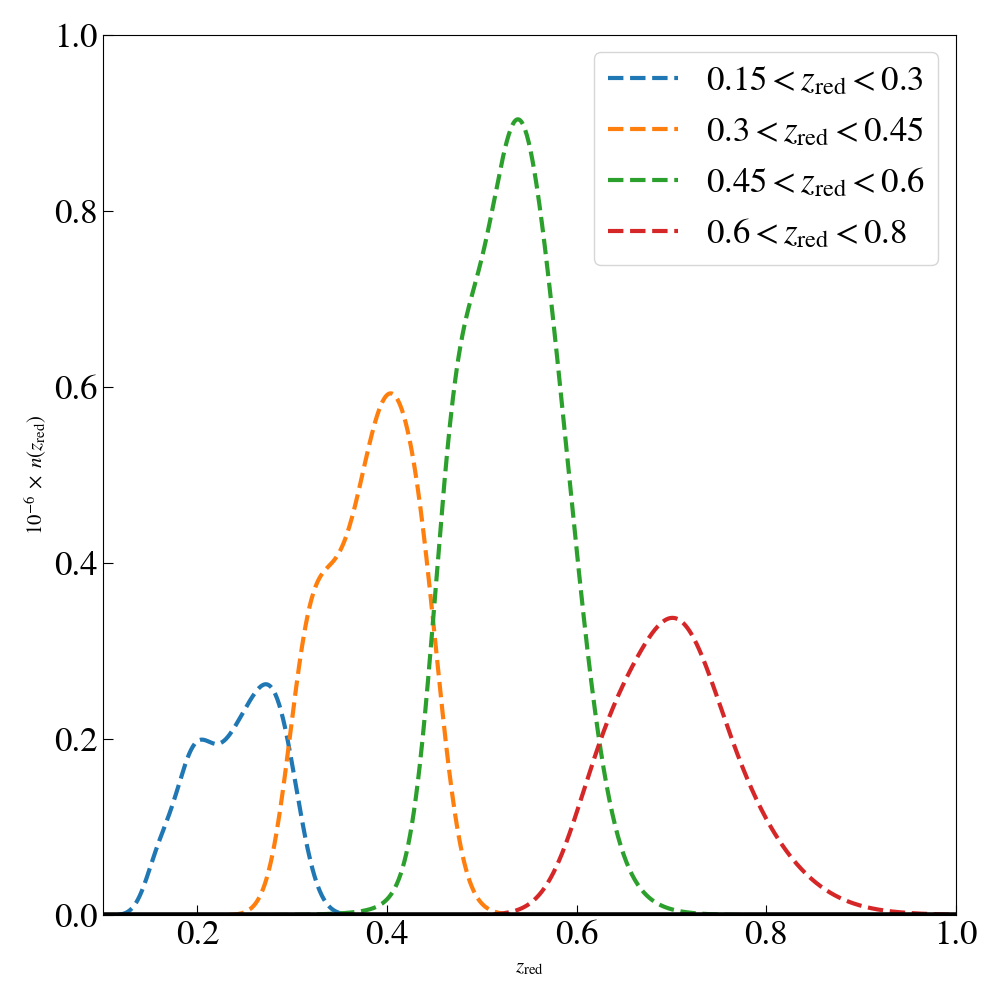
\includegraphics[width=\columnwidth]{figures_tmp/nofz.png}
%\caption{\label{fig:pz} Tomographic redshift distributions of our red galaxy sample in four bins: %$0.15<z_{\rm red}<0.3, \;0.3<z_{\rm red}<0.45, \;0.45<z_{\rm red}<0.6, \;0.6<z_{\rm red}<0.8$.
% The redshift distributions of the lenses are estimated directly from the the individual red-sequence %redshift estimates and their corresponding uncertainties.} 
%\end{figure}



\begin{figure*}
\begin{tabular}{cc}
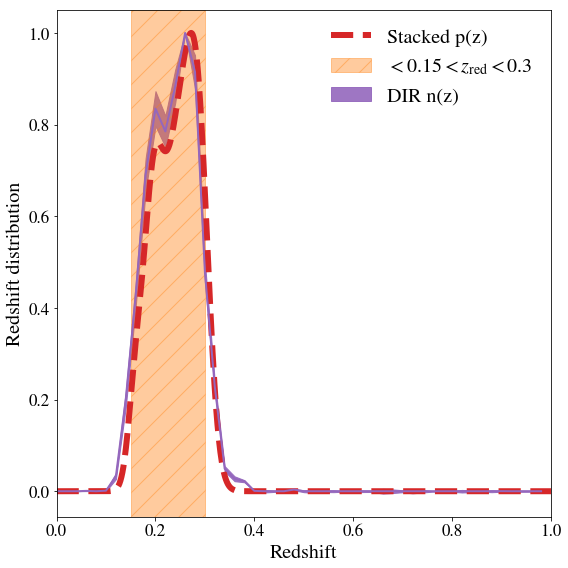
\includegraphics[width=\columnwidth]{figures_tmp/nz_comp_1.png}
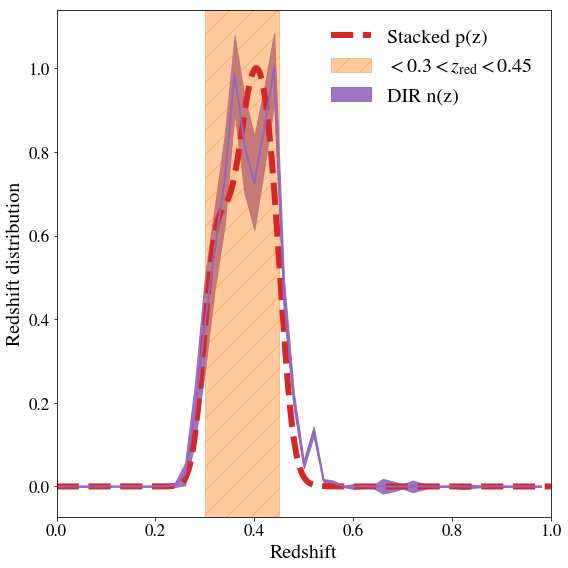
\includegraphics[width=\columnwidth]{figures_tmp/nz_comp_2.png}
\end{tabular}
\begin{tabular}{cc}
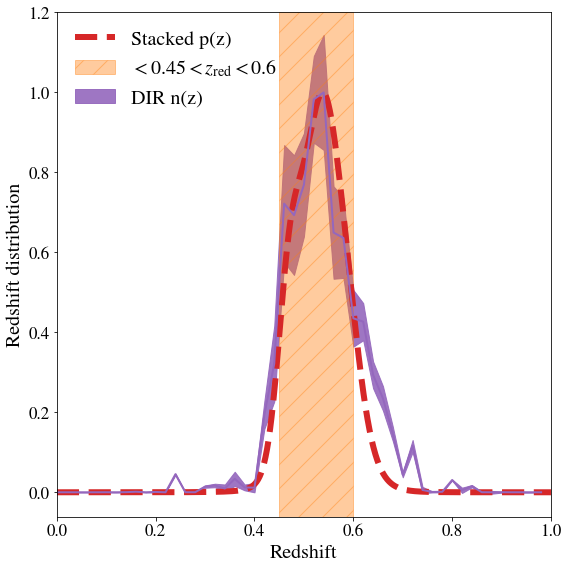
\includegraphics[width=\columnwidth]{figures_tmp/nz_comp_3.png}
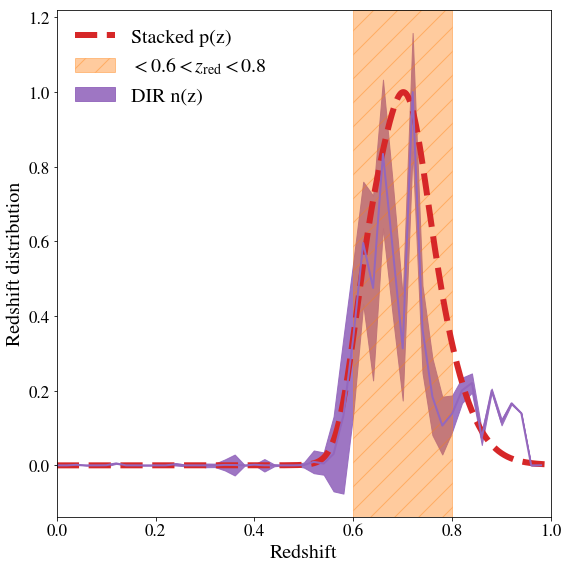
\includegraphics[width=\columnwidth]{figures_tmp/nz_comp_4.png}
\end{tabular}

\caption{\label{fig:pz2} Tomographic redshift distributions of our red galaxy sample in four bins: $0.15<z_{\rm red}<0.3, \;0.3<z_{\rm red}<0.45, \;0.45<z_{\rm red}<0.6, \;0.6<z_{\rm red}<0.8$.
 The redshift distributions are estimated from two methods: DIR redshift distributions are shown in blue and the stacked redshift probabilities are shown in orange.} 
\end{figure*}




\begin{figure*}
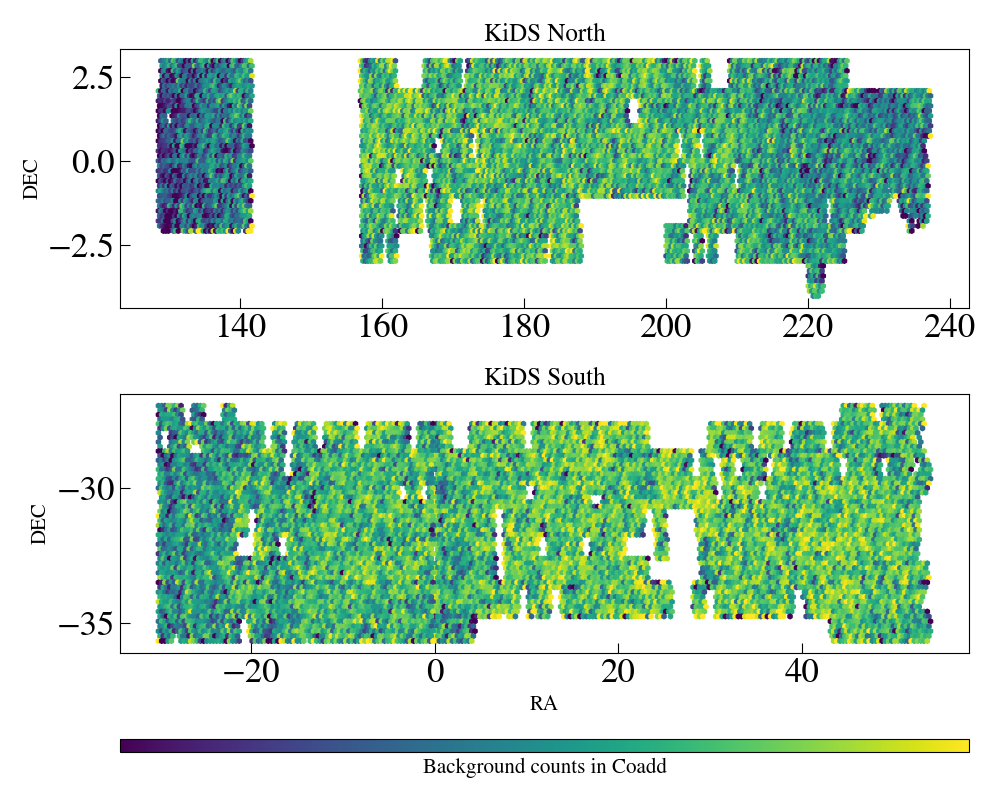
\includegraphics[width=\textwidth]{figures_tmp/sys/scatter_BackGr.png}
\caption{\label{fig:scatter_BackGr} The healpix map of the background counts in the coadded images in the $r$-band in the KiDS DR4 footprint.} 
\end{figure*}

\begin{figure*}
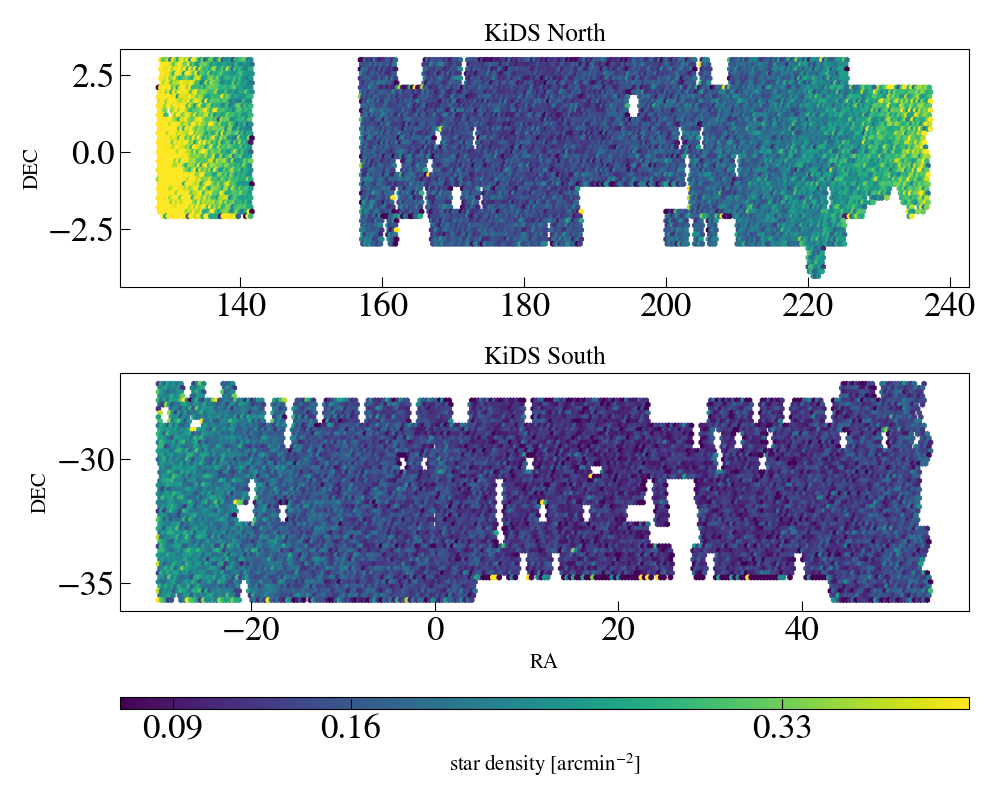
\includegraphics[width=\textwidth]{figures_tmp/sys/scatter_nstar.png}
\caption{\label{fig:scatter_stardens} The healpix map of the density of GAIA DR2 stars ($14<G<17$) in the KiDS DR4 footprint.} 
\end{figure*}

\begin{figure*}
\begin{tabular}{cc}
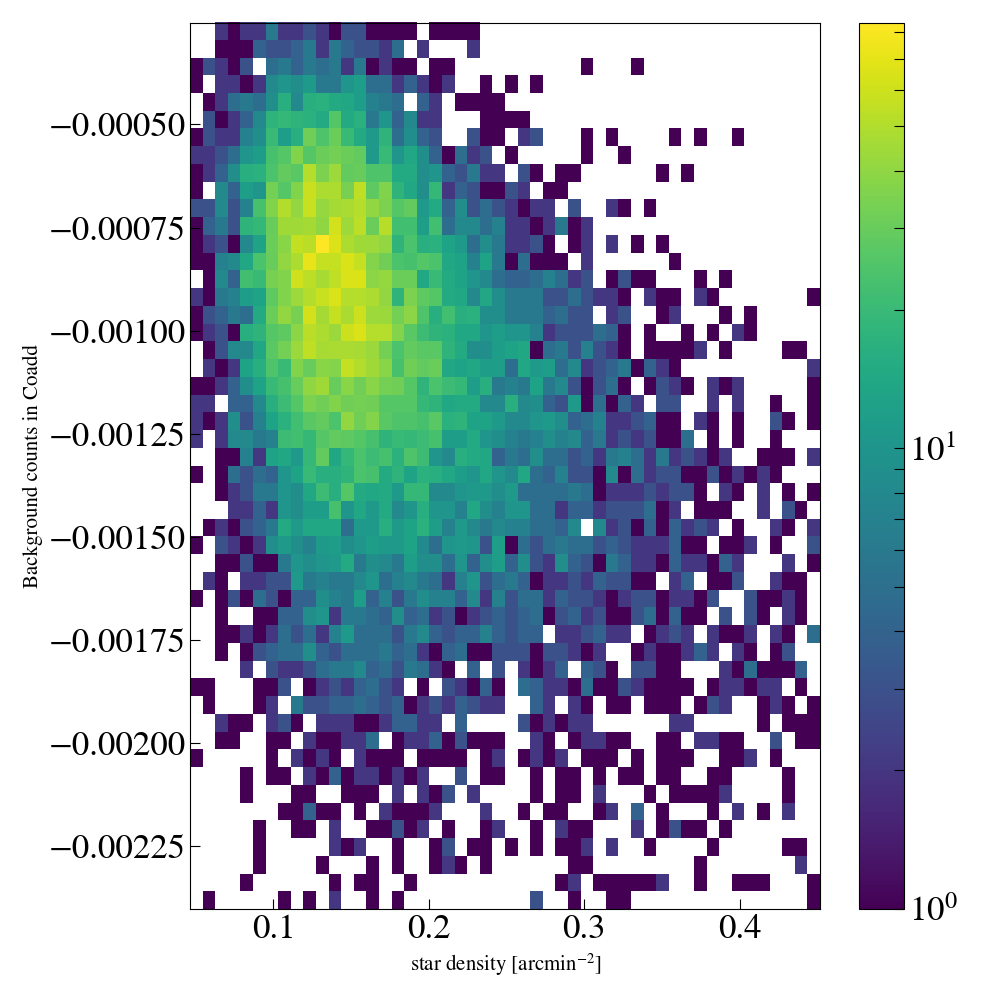
\includegraphics[width=0.5\textwidth]{figures_tmp/sys/correlation1.png}
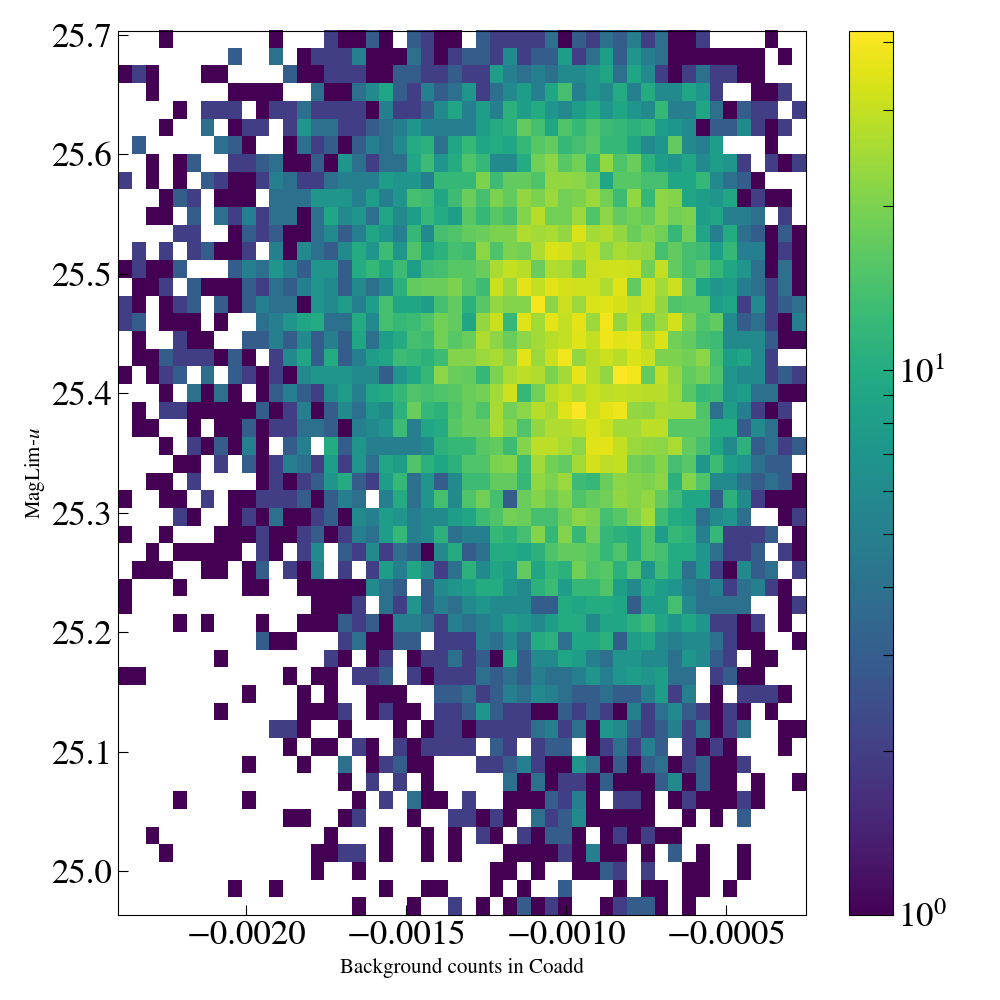
\includegraphics[width=0.5\textwidth]{figures_tmp/sys/correlation2.png}
\end{tabular}
\begin{tabular}{cc}
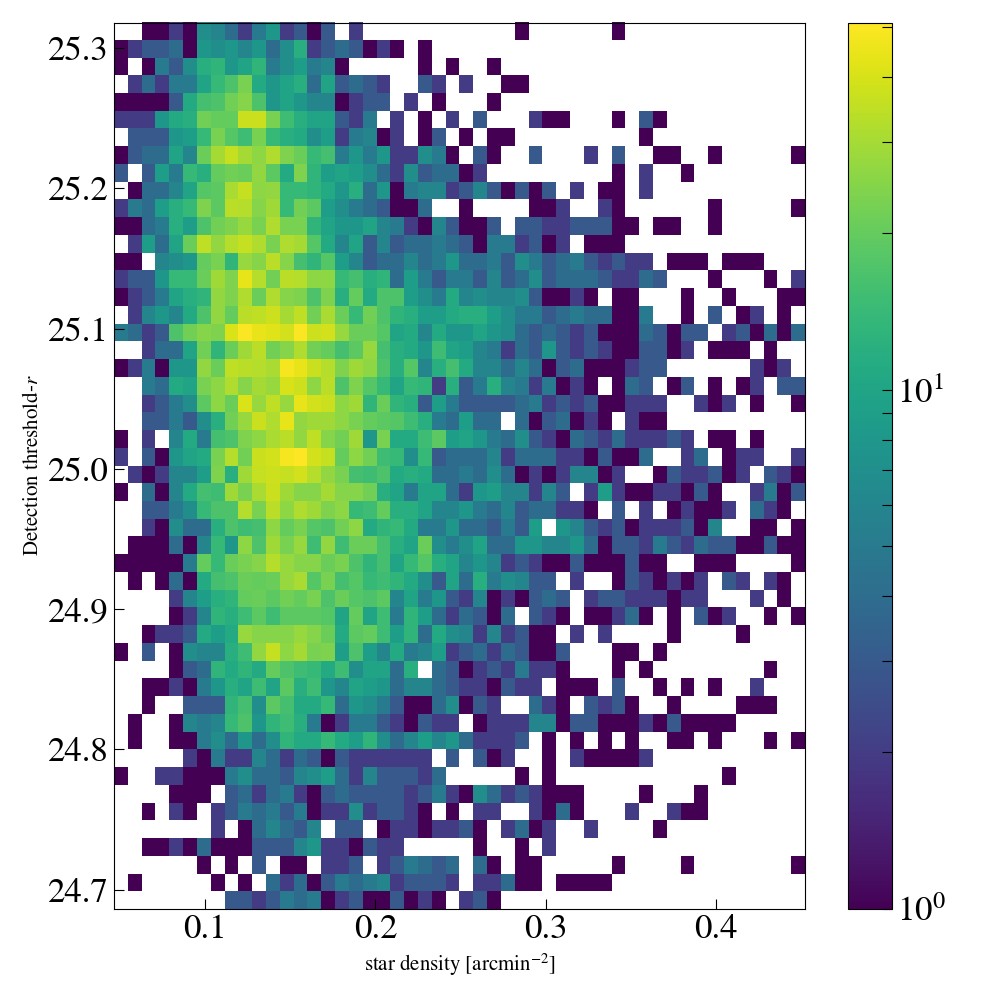
\includegraphics[width=0.5\textwidth]{figures_tmp/sys/correlation3.png}
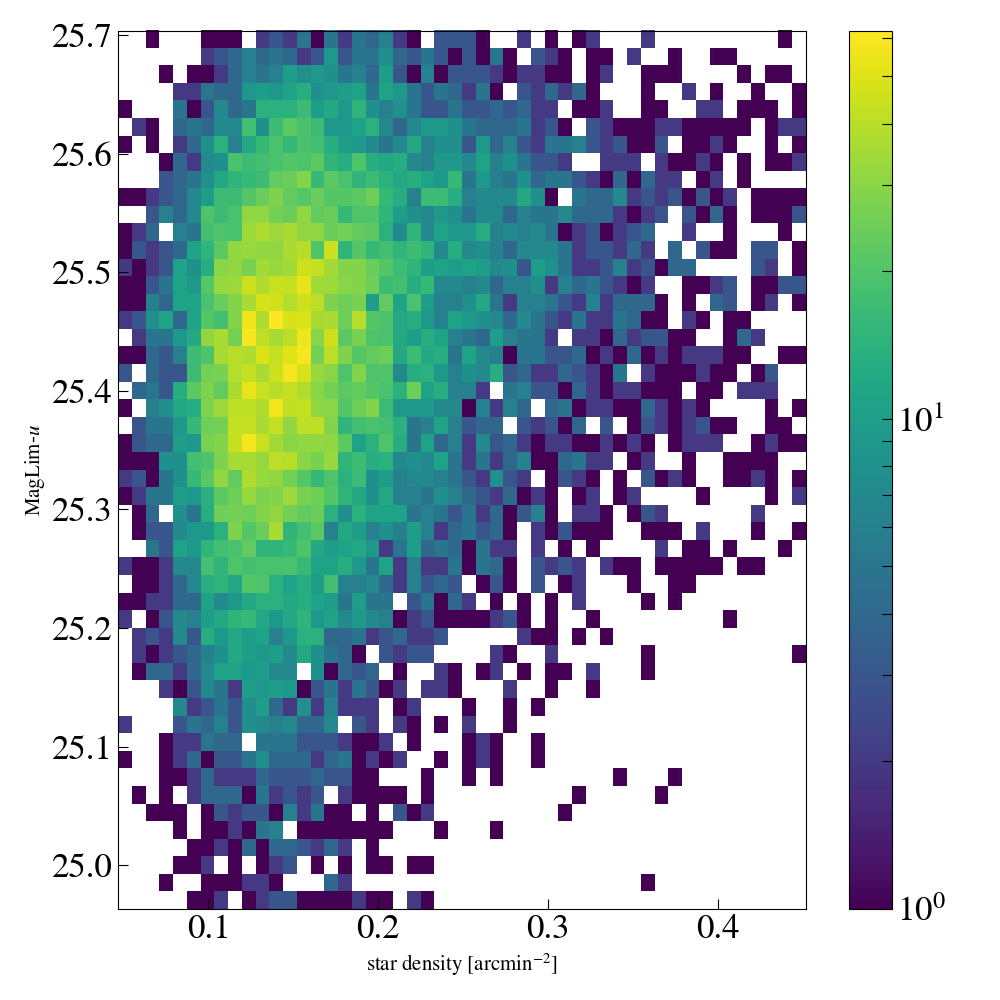
\includegraphics[width=0.5\textwidth]{figures_tmp/sys/correlation5.png}
\end{tabular}
\caption{\label{fig:sys_sys_correlation} Demonstration of the non-negligible covariance between the survey properties. The anti-correlation between the Background counts in the coadds and the stellar number density is evident (\textit{Top Right}). Furthermore, we note the anti-correlation between the magnitude limit in the $u$-band (\textit{Top Right}), anti-correlation between the detection threshold and the star number density (\textit{Bottom Left}), and the magnitude limit in the $u$-band and the star number density (\textit{Bottom Right}).} 
\end{figure*}


\begin{figure*}
\begin{tabular}{ccc}
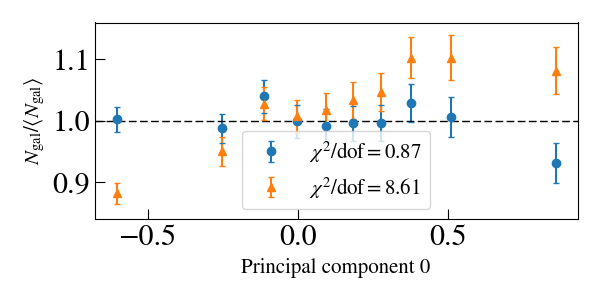
\includegraphics[width=0.3\textwidth]{figures_tmp/sys/result_pca_ngal_0_15_0_poly_1.png}
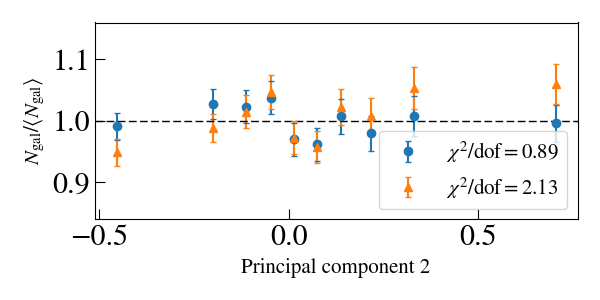
\includegraphics[width=0.3\textwidth]{figures_tmp/sys/result_pca_ngal_0_15_2_poly_1.png}
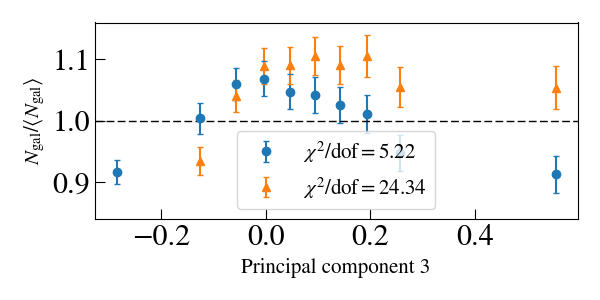
\includegraphics[width=0.3\textwidth]{figures_tmp/sys/result_pca_ngal_0_15_3_poly_1.png}
\end{tabular}

\begin{tabular}{ccc}
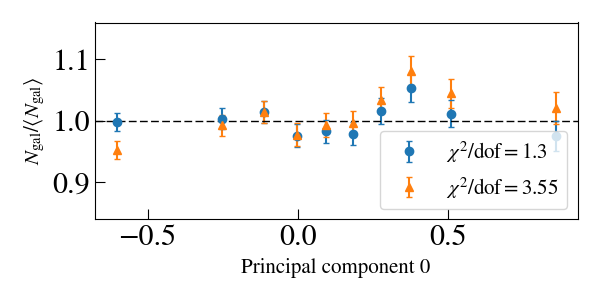
\includegraphics[width=0.3\textwidth]{figures_tmp/sys/result_pca_ngal_0_3_0_poly_1.png}
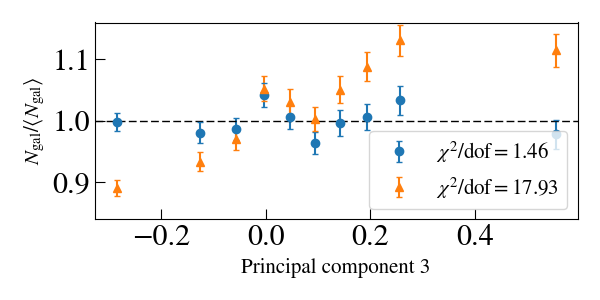
\includegraphics[width=0.3\textwidth]{figures_tmp/sys/result_pca_ngal_0_3_3_poly_1.png}
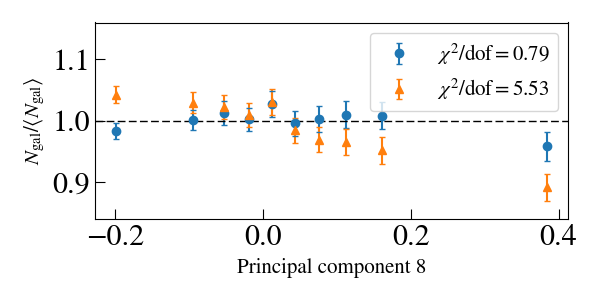
\includegraphics[width=0.3\textwidth]{figures_tmp/sys/result_pca_ngal_0_3_8_poly_1.png}
\end{tabular}

\begin{tabular}{ccc}
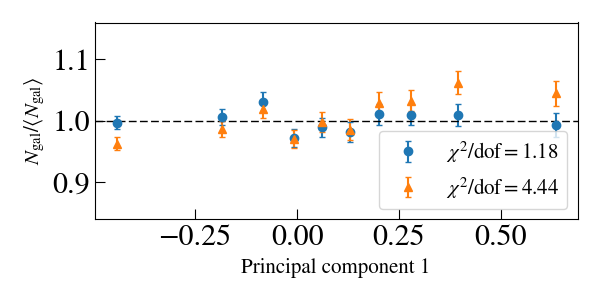
\includegraphics[width=0.3\textwidth]{figures_tmp/sys/result_pca_ngal_0_45_1_poly_1.png}
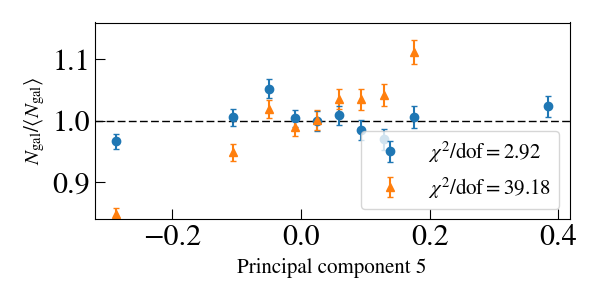
\includegraphics[width=0.3\textwidth]{figures_tmp/sys/result_pca_ngal_0_45_5_poly_1.png}
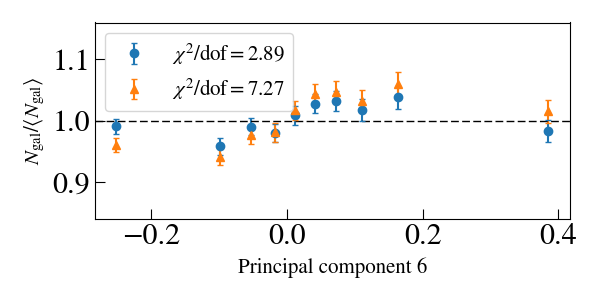
\includegraphics[width=0.3\textwidth]{figures_tmp/sys/result_pca_ngal_0_45_6_poly_1.png}
\end{tabular}

\begin{tabular}{ccc}
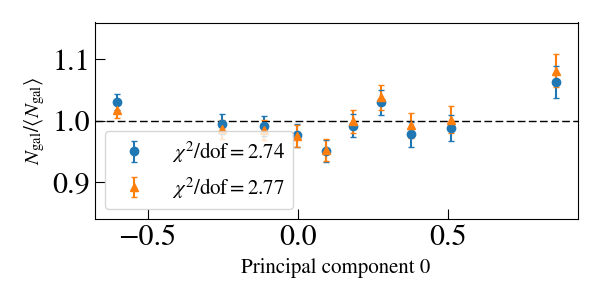
\includegraphics[width=0.3\textwidth]{figures_tmp/sys/result_pca_ngal_0_6_0_poly_1.png}
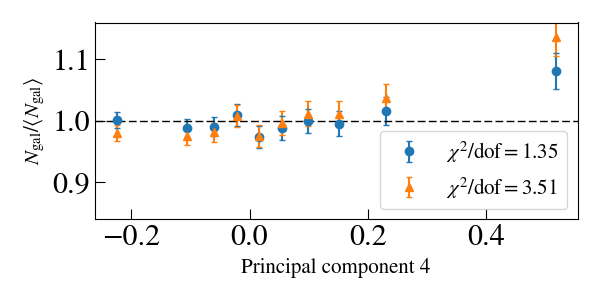
\includegraphics[width=0.3\textwidth]{figures_tmp/sys/result_pca_ngal_0_6_4_poly_1.png}
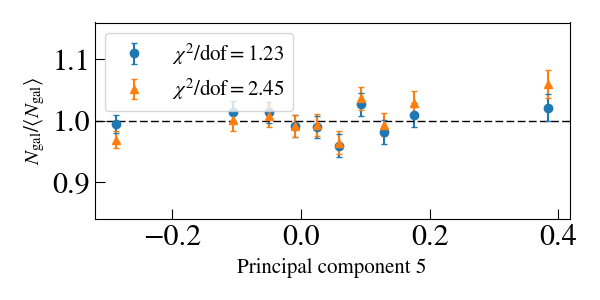
\includegraphics[width=0.3\textwidth]{figures_tmp/sys/result_pca_ngal_0_6_5_poly_1.png}
\end{tabular}

\caption{\label{fig:sys_ng_correlation} Demonstration of the correlation between the observed galaxy number densities and the principal components of the survey properties before (shown in orange) and after the application of systematic weights (shown in blue). The panels from top to bottom show the systematic correlation in the $0.15<z_{\rm red}<0.3$, $0.3<z_{\rm red}<0.45$, $0.45<z_{\rm red}<0.6$, $0.6<z_{\rm red}<0.8$ tomographic bins respectively. In each row, a subset of principal components that exhibit considerable correlation with the observed number densities are shown.} 
\end{figure*}

\begin{figure*}
\begin{tabular}{c}
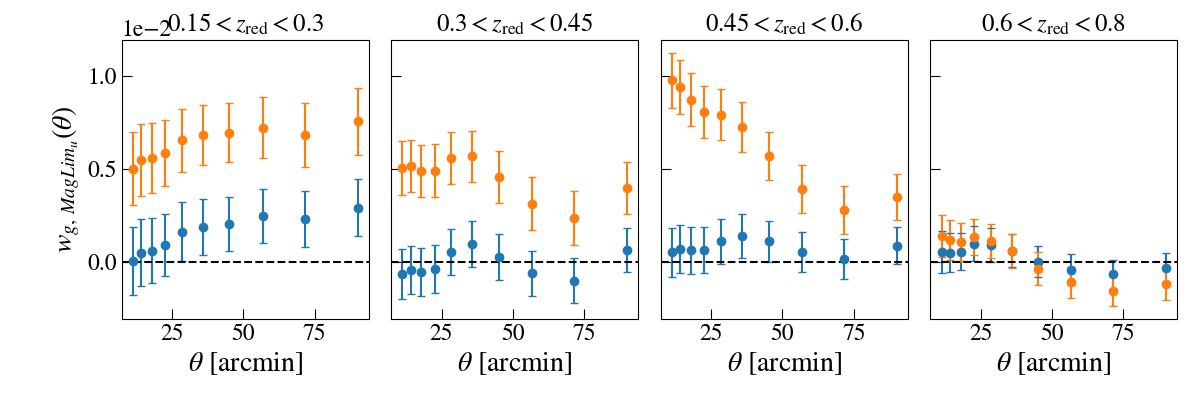
\includegraphics[width=\textwidth]{figures_tmp/sys/wcross_sys_type_ulim.png}
\end{tabular}
\begin{tabular}{c}
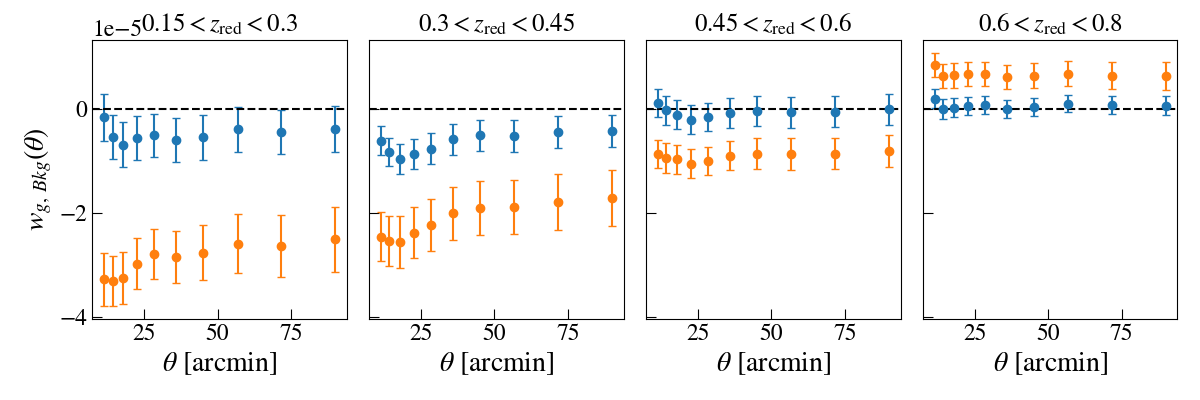
\includegraphics[width=\textwidth]{figures_tmp/sys/wcross_sys_type_BackGr.png}
\end{tabular}
\caption{\label{fig:xcorr_ulim_bkg}} 
\end{figure*}

\begin{figure*}
\begin{tabular}{c}
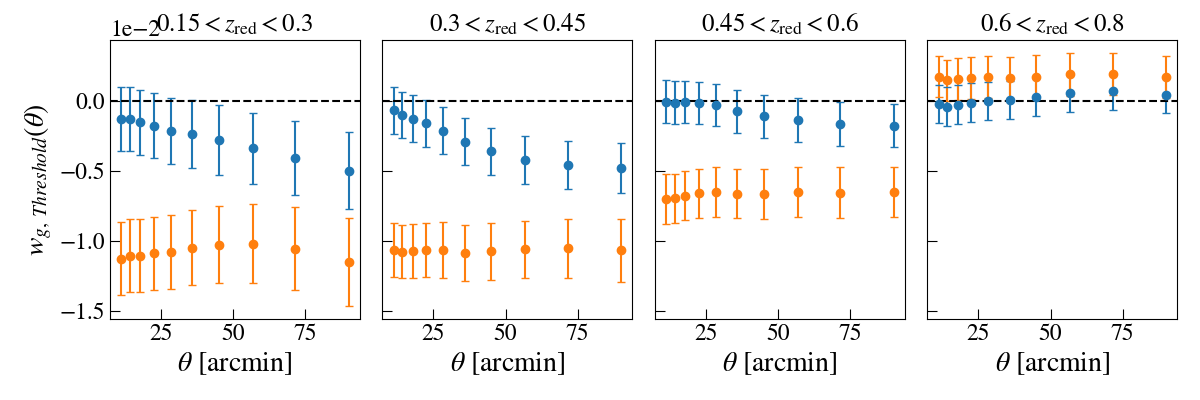
\includegraphics[width=\textwidth]{figures_tmp/sys/wcross_sys_type_threshold.png}
\end{tabular}
\begin{tabular}{c}
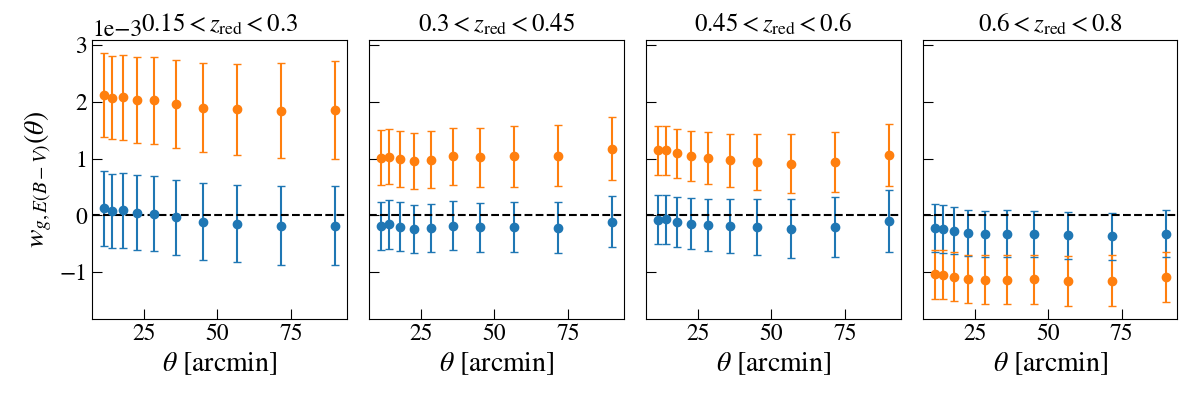
\includegraphics[width=\textwidth]{figures_tmp/sys/wcross_sys_type_extinction.png}
\end{tabular}
\caption{\label{fig:xcorr_threshold_ext}} 
\end{figure*}


\begin{figure*}
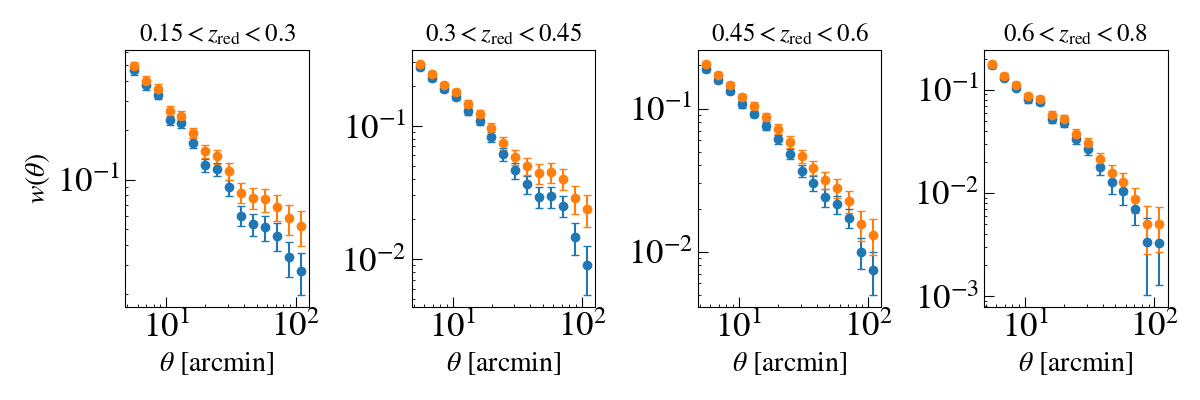
\includegraphics[width=\textwidth]{figures_tmp/xi.png}
\caption{\label{fig:xi} Clustering measurements for the four tomographic bins. In each panel, the blue (orange) data-points correspond to the 2PCF computed with (without) the systematic weights.} 
\end{figure*}


\begin{figure*}
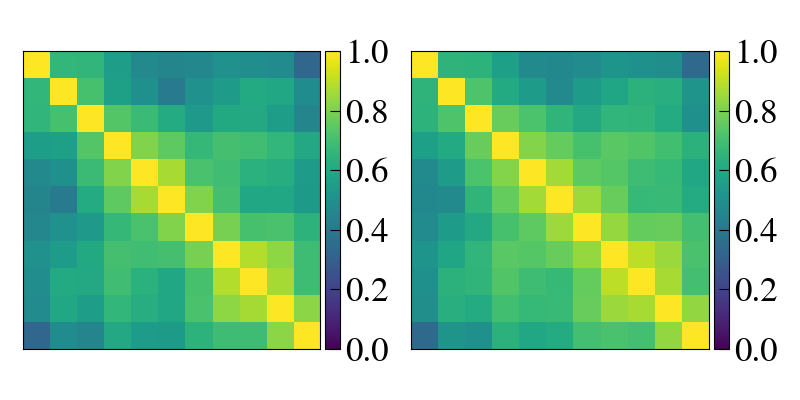
\includegraphics[width=\textwidth]{figures_tmp/correlation_0_6.png}
\caption{\label{fig:xi} Two correlation matrix corresponding to the angular clustering measurements in the last tomographic bin. One of the matrices is the original correlation matrix derived from the jackknife covariance matrix computed in section~\ref{sec:measurement}, while the other matrix is constructed with the method of~\citet{sellentin2019} such that the posterior value picks at some predefined value.} 
\end{figure*}

\begin{figure*}
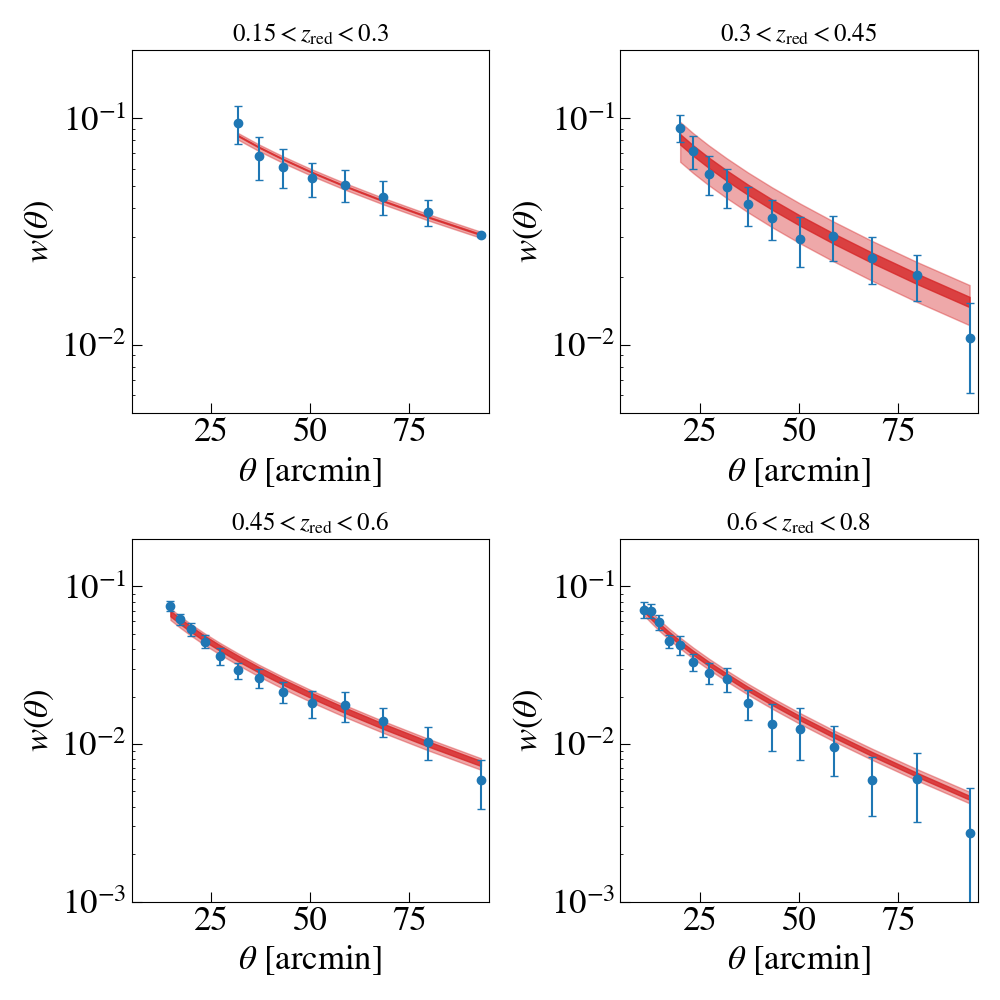
\includegraphics[width=\textwidth]{figures_tmp/w_estimate.png}
\caption{\label{fig:xi} Comparison between the posterior predictions (red shaded) of clustering and the clustering measurements (blue) in the four tomographic bins. The dark and light shaded regions mark the 68\% and the 95\% confidence intervals. The error bars are from the diagonal elements of the blinded covariance matrix of the observations.} 
\end{figure*}


\begin{figure}
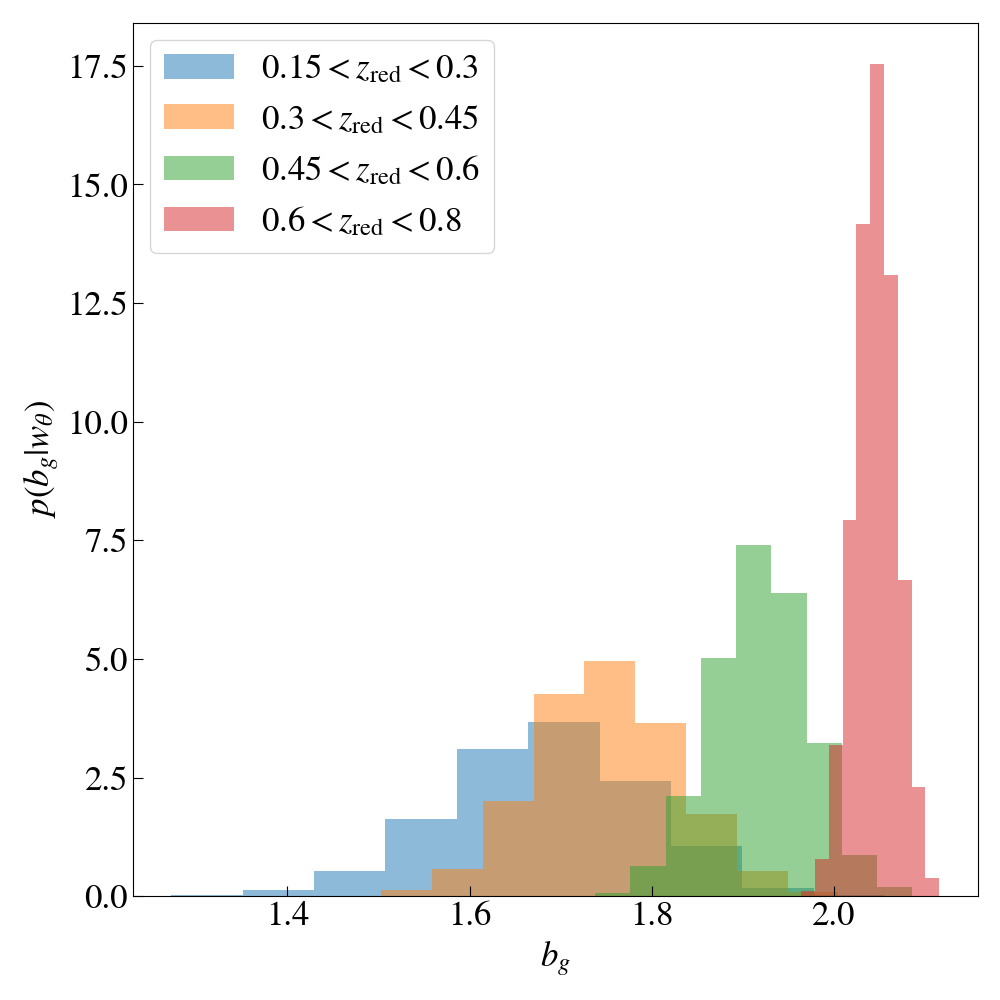
\includegraphics[width=\columnwidth]{figures_tmp/b_estimate.png}
\caption{\label{fig:xi} Constraints on the linear galaxy bias of the red-sequence sample in four tomographic bins.} 
\end{figure}



%%%%%%%%%%%%%%%%%%%%%%%%%%%%%%%%%%%%%%%%%%%%%%%%%%

%%%%%%%%%%%%%%%%%%%% REFERENCES %%%%%%%%%%%%%%%%%%
% BibTeX:

\bibliographystyle{mnras}
\bibliography{lrg_kids.bib}

%%%%%%%%%%%%%%%%%%%%%%%%%%%%%%%%%%%%%%%%%%%%%%%%%%

%%%%%%%%%%%%%%%%% APPENDICES %%%%%%%%%%%%%%%%%%%%%
%\clearpage

\appendix


\bsp	% typesetting comment
\label{lastpage}
\end{document}
